\documentclass[a4paper,twocolumn,11pt]{quantumarticle}
\pdfoutput=1

\usepackage[utf8]{inputenc}
\usepackage[english]{babel}
\usepackage[T1]{fontenc}
\usepackage{amsmath, amssymb, amsfonts}

\usepackage{microtype}
\usepackage{braket}
\usepackage{tikz}
\usepackage{tabularx}
\usepackage{makecell}
\usepackage{graphicx}
\graphicspath{{figures/}{../figures/}}

\newtheorem{theorem}{Theorem}

\begin{document}

\title{Control-Space Scaling of Correlated Phase Networks in Parallel Spin Shuttling Architectures}

\author{Inuk You}
\email{youinuk@gmail.com}
\affiliation{Department of Science, Kyungdong High School, Seoul 02870, Republic of Korea}

\begin{abstract}
Scalable semiconductor spin-qubit architectures increasingly rely on electron shuttling for non-local connectivity. In dense parallel transport, however, shuttling-induced phase accumulation is not well described as a set of independent local rotations. We show that spatially correlated electromagnetic fields generate a dense, deterministic relative-phase network among simultaneously moving qubits. In the modeled dense-routing regime, the associated susceptibility matrix remains near full rank and therefore presents an $O(K^2)$ pairwise calibration burden for an active register of size $K$.

We introduce a hardware-software co-design framework that addresses this bottleneck through multiplexed Ramsey probing and software-level virtual-Z compensation. The reduction in experimental round count originates from the parallel probing protocol: each Ramsey experiment applies a randomized displacement vector and reads out all active qubit phases in parallel, turning pairwise calibration into a system-identification problem. A physics-informed $1/r^3$ structural prior is used to decompose the reconstructed susceptibility matrix into a geometric baseline and residual device-specific correction; in the overdetermined regime studied here, it should be interpreted as a physically meaningful coordinate system rather than as the primary source of statistical speedup.

Under idealized parallel probing conditions and the normalized simulation model used throughout this work, $n_{\rm exp}=2K$ independent Ramsey rounds are empirically sufficient to reconstruct the susceptibility matrix for high-fidelity virtual-Z compensation. The compensated simulations maintain $F_{\rm comp}>0.999$ over the tested range and avoid the sequential pairwise drift wall near $K\approx30$ under the assumed timing model. These results should be read as reference scaling limits for dense spin-shuttling control, rather than as device-specific fidelity predictions.
\end{abstract}

\maketitle

\section{Introduction}

The scalability of semiconductor spin qubits has emerged as a central challenge in the pursuit of large-scale quantum processors \cite{vandersypen_interfacing_2017}. Silicon-based spin qubits offer long coherence times and have demonstrated high-fidelity gate operations in small registers \cite{reiner_high-fidelity_2024, kim_quantum_2014}. They also allow for accurate tomography of exchange-coupled logic \cite{stemp_tomography_2024}. Furthermore, their compatibility with advanced VLSI manufacturing \cite{meunier_silicon_2025} and 300~mm industrial CMOS wafer processes \cite{koch_industrial_2025} positions them as a highly promising platform for fault-tolerant computation \cite{watson_programmable_2018, aharonov_fault-tolerant_2008}. 

Yet, scalability ultimately hinges on connectivity; the physical movement of quantum information across extended qubit arrays remains a fundamental bottleneck \cite{burkard_semiconductor_2023, hu_single-electron_2025}. Electron spin shuttling has recently been demonstrated as a key architectural primitive to enable long-range connectivity beyond nearest-neighbor constraints \cite{mills_shuttling_2019, seidler_conveyor-mode_2022}. Recent advances have showcased baseband control in 2D arrays \cite{unseld_baseband_2025}, the implementation of shared control to efficiently operate crossbar arrays \cite{borsoi_shared_2024}, and the distribution of entanglement between distant sub-modules \cite{ademi_distributing_2026}. 

Recent demonstrations of shuttling-enabled gates between distant processors \cite{noiri_shuttling-based_2022} and two-qubit logic on mobile spins \cite{matsumoto_two-qubit_2025} indicate that relative phase coherence during transport will become a central control requirement. This requirement is especially relevant when mobile-spin operations are combined with high-fidelity exchange control in industrial platforms \cite{chittock-wood_radio-frequency_2024}.

The usual approximation that shuttling-induced dynamical phases can be treated as independent, local single-qubit rotations \cite{de_smet_high-fidelity_2025} becomes incomplete in dense two-dimensional arrays. When many qubits are transported simultaneously, spatially structured control fields, electrostatic crosstalk, and anisotropic $g$-tensor effects \cite{geyer_anisotropic_2024, fedele_simultaneous_2021} generate correlated phase shifts. The resulting object is a dense deterministic phase network, rather than a collection of independent local stochastic errors \cite{cifuentes_impact_2024, jin_probing_2024, blume-kohout_demonstration_2017, wilen_correlated_2021}.

This spatial correlation creates a calibration burden that grows rapidly with the number of simultaneously routed qubits. Unlike independent local phase offsets, correlated accumulation requires estimating relative phases across many pairs; in the dense limit, the susceptibility matrix contains $O(K^2)$ relevant off-diagonal entries. This motivates a scalable inference-and-compensation strategy rather than independent calibration of each moving spin or direct analytical control over all pairwise phases \cite{tanttu_assessment_2024, proctor_benchmarking_2025, glaser_training_2015}.

To overcome this architectural barrier, we propose a multiplexed inference and software-level compensation strategy. Instead of attempting to physically eliminate all correlated phases through increasingly isolated hardware, our framework (Fig.~\ref{fig:figure1}) treats the deterministic phase network as an experimentally identifiable susceptibility matrix. Multiplexed Ramsey-based system identification \cite{ruffino_cryo-cmos_2022, harper_efficient_2020} acquires parallel phase responses to randomized displacement probes, while a physics-informed decomposition organizes the recovered operator into a geometric $1/r^3$ baseline and a residual device-specific correction. The resulting surrogate is then used by the compiler to apply virtual Z-rotations, compensating transport-induced relative phases without adding physical microwave operations.

Specifically, our contributions are fourfold: 
(1) we develop a theoretical framework for phase dynamics in mobile spin-qubit architectures and identify the emergence of deterministic spatial correlations; 
(2) we derive a transport-induced phase susceptibility model showing why dense parallel shuttling generically creates an $O(K^2)$ calibration space; 
(3) we demonstrate, within an idealized parallel Ramsey probing model, that multiplexed system identification can reduce the required number of calibration rounds to $O(K)$; and 
(4) we show that the reconstructed susceptibility network can be used for software-level virtual-Z compensation, with a $1/r^3$ structural prior providing an interpretable baseline-residual decomposition rather than the primary source of the scaling reduction.

\paragraph{Scope and assumptions.}
The numerical results in this work are intended as reference scaling limits for a normalized dense-shuttling model. The reported values, including $F_{\text{comp}}>0.999$, $n_{\rm exp}=2K$, and the drift-wall scale near $K\approx30$, assume idealized parallel phase readout, the stated projection-noise model, randomized routing displacements, and a simplified sequential timing model for the pairwise baseline. They should therefore be interpreted as evidence for the structural viability of multiplexed inference and software compensation, not as device-faithful predictions for a particular chip.

\paragraph{Relation to existing calibration and control strategies.}
The present work is complementary to local shuttling-phase calibration, static crosstalk characterization, randomized multiplexed measurement, and numerical optimal-control approaches \cite{de_smet_high-fidelity_2025, tanttu_assessment_2024, ruffino_cryo-cmos_2022, harper_efficient_2020, proctor_benchmarking_2025, glaser_training_2015}. Its distinction is not the introduction of a new physical gate, but the treatment of transport-induced phase shifts as a dense, deterministic susceptibility network that can be inferred through vector-valued Ramsey responses and then tracked in software. This positioning also clarifies the role of the $1/r^3$ prior: it supplies a physically meaningful baseline for interpreting the recovered matrix, whereas the experimental round-count reduction in the demonstrated regime comes from multiplexed probing.

\paragraph{Generality.}
Although the microscopic derivations are framed around electron spins navigating nanomagnet stray fields, the same modeling logic may apply to other mobile solid-state qubit platforms in which routing through spatially varying frequency or spin-orbit landscapes produces deterministic, geometry-dependent phase responses. Examples include hole-spin devices with strong spin-orbit coupling and anisotropic noise or exchange response, as well as dense CMOS-style dot arrays where electrostatic crosstalk can shift spin resonance frequencies \cite{hendrickx_sweet-spot_2024, geyer_anisotropic_2024, cifuentes_impact_2024}. More broadly, the scaling motivation is aligned with semiconductor spin-qubit architectures that rely on dense integration, shared control, and CMOS-compatible routing infrastructure \cite{burkard_semiconductor_2023, gonzalez-zalba_scaling_2021, borsoi_shared_2024}. The quantitative thresholds reported below, however, are tied to the adopted nanomagnet-inspired reference model and should not be read as general performance guarantees.


\begin{figure*}[!htbp]
\centering
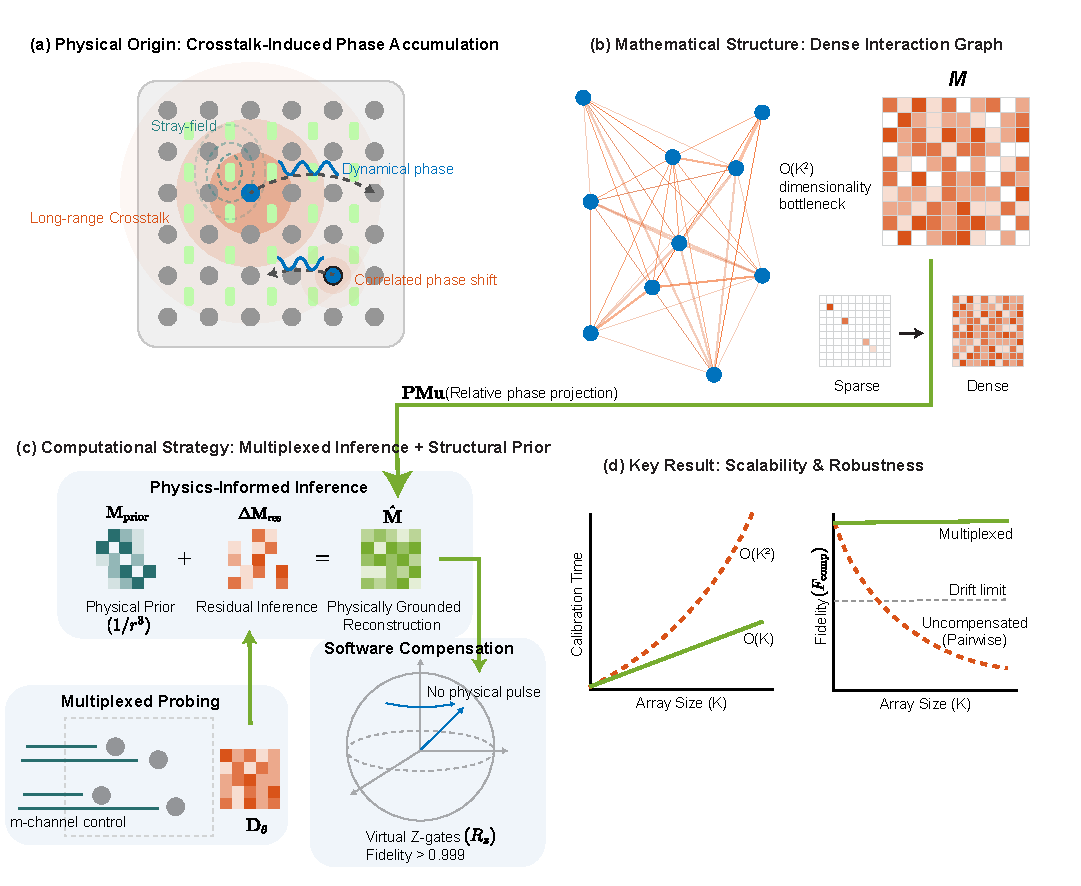
\includegraphics[width=\textwidth]{fig_1.pdf}
\caption{\textbf{Conceptual overview of the hardware-software co-design for correlated phase tracking.}
(a) Physical origin of shuttling-induced correlated phase dynamics. Parallel transport of multiple spin qubits (blue spheres) through periodic nanomagnet arrays (teal) subjects them to trajectory-dependent magnetic field variations. This motion induces accumulated dynamical phase variations (blue sine waves) on individual trajectories. Concurrently, the algebraically decaying stray fields facilitate long-range crosstalk (red), where the displacement of one qubit induces a correlated phase shift on its neighbors, forming a dense, deterministic error network.
(b) Dimensionality bottleneck in the interaction graph. The spatial correlation among moving qubits forms a highly connected interaction network (left), which mathematically manifests as a dense susceptibility operator $\mathbf{M}$ (right heatmap). Incorrectly assuming localized interactions yields an artificially sparse parameter space (bottom left inset). In reality, the $1/r^3$ dipolar interaction fills the off-diagonal elements (bottom right inset), leading to an $O(K^2)$ expansion that acts as a major scalability bottleneck for sequential calibration.
(c) Scalable compensation strategy via multiplexed inference. To address this bottleneck, multiplexed probing (bottom left) acquires parallel phase data ($\mathbf{D}_\theta$) from simultaneously active qubits via $m$-channel parallel control. An inference engine (top) reconstructs the susceptibility operator and organizes it into a geometric baseline ($\mathbf M_{\rm prior}$, teal) and a data-driven residual correction operator ($\Delta\mathbf M_{\rm res}$, red). In the overdetermined regime studied here, this decomposition provides physical interpretability, while the reduction in calibration rounds comes from multiplexed probing. The inferred corrections are applied via virtual Z-gates (bottom right) at the compiler level, rotating the computational frame without additional physical control operations.
(d) Benchmarking scalability and robustness. Under the normalized simulation model, the proposed framework maintains a compensation fidelity $F_{\text{comp}} > 0.999$ throughout the explored range of array sizes (green curve, right plot). This multiplexed approach achieves linear $O(K)$ scaling in calibration time (left plot), avoiding the quadratic $O(K^2)$ overhead of pairwise calibration under the assumed timing model and remaining within representative hardware drift constraints (grey dashed line). Schematic not to scale.}
\label{fig:figure1}
\end{figure*}


\subsection*{Notation and principal quantities}
For clarity, Table~\ref{tab:notation} summarizes the principal symbols used throughout the theory, simulations, and figure captions. Unless otherwise stated, the numerical results are reported in the normalized units of the simulation model.

\begin{table*}[t!]
\centering
\caption{Notation and principal quantities. The distinction between the physical phase-dispersion objective and the compensation-fidelity residual is important: trajectory optimization acts on $\|P\hat{\mathbf M}\mathbf u\|^2$, whereas $F_{\rm comp}$ evaluates the residual phase after virtual-Z correction, $P(\mathbf M-\hat{\mathbf M})\mathbf u$.}
\label{tab:notation}
\renewcommand{\arraystretch}{1.1}
\begin{tabular}{lll}
\hline
Symbol & Meaning & Used in \\
\hline
$K$ & Number of simultaneously shuttled active qubits & scaling and calibration cost \\
$a$ & Lattice pitch; simulation length unit & geometry and distance scaling \\
$\mathbf r_i(t)$ & Trajectory of qubit $i$ during transport & phase-dynamics model \\
$\chi_{ij}$ & \makecell[l]{Spatial susceptibility kernel coupling \\ displacement of $j$ to phase of $i$} & physical crosstalk model \\
$\mathbf M$ & Dense transport-induced phase susceptibility matrix & rank analysis and inference \\
$(M_{\rm prior})_{ij}$ & Ideal geometric $1/r^3$ baseline susceptibility & baseline--residual decomposition \\
$\Delta\mathbf M_{\rm res}$ & \makecell[l]{Residual correction in \\ $\mathbf M=\mathbf M_{\rm prior}+\Delta\mathbf M_{\rm res}$} & device-specific deviation \\
$\hat{\mathbf M}$ & \makecell[l]{Reconstructed susceptibility matrix \\ estimated from Ramsey data} & virtual-Z compensation \\
$\mathbf u$ & \makecell[l]{Vector of shuttling displacements or \\ displacement-like probe amplitudes} & calibration and routing \\
$U_J$ & \makecell[l]{Nominal displacement scale, \\ $U_J=X_{\max}T_{\rm trans}/2$} & probe and routing amplitude \\
$\mathbf U$ & \makecell[l]{Calibration design matrix containing \\ $n_{\rm exp}$ probe vectors} & multiplexed inference \\
$\mathbf D_{\rm ideal}$ & \makecell[l]{Ideal deterministic phase-response matrix \\ before injected noise and bandwidth limits} & operational validation \\
$\mathbf D_\theta$ & \makecell[l]{Stacked Ramsey phase-response matrix \\ over $n_{\rm exp}$ probe rounds} & multiplexed inference \\
$\Delta\boldsymbol\theta$ & Measured vector of Ramsey phase responses & observation model \\
$n_{\rm exp}$ & Number of independent Ramsey calibration rounds & experimental overhead \\
$m$ & \makecell[l]{Number of nonzero probe displacements \\ in a sub-array round} & bandwidth-constrained robustness \\
$P$ & \makecell[l]{Gauge projector $I-\mathbf 1\mathbf 1^{T}/K$ \\ removing global phase} & relative phase metrics \\
$r_\varepsilon$ & Effective rank at singular-value threshold $\varepsilon$ & Stage-1 bottleneck analysis \\
$F_{\rm comp}$ & \makecell[l]{Compensation fidelity \\ $\exp[-\|P(\mathbf M-\hat{\mathbf M})\mathbf u\|^2/2(K-1)]$} & virtual-Z performance metric \\
$\alpha$ & Structural prior-mismatch amplitude & robustness validation \\
$\sigma_\varphi$ & Ramsey projection-noise standard deviation & measurement noise \\
$\sigma_{\rm self}$ & Residual self-phase-noise standard deviation & stochastic robustness validation \\
$\sigma_M$ & Single-entry matrix uncertainty, $\sigma_\varphi/U_J$ & SNR and FT-relevance analysis \\
$\kappa(\mathbf U)$ & Probe-design condition number & inference stability diagnostic \\
$T_{\rm Ramsey}$ & Wall-clock time assigned to one Ramsey round & calibration time model \\
$T_{\rm cal}$ & \makecell[l]{Total wall-clock calibration time \\ under the assumed timing model} & operational metric extraction \\
$\tau_{\rm drift}$ & Representative calibration-stability window & drift-wall comparison \\
\hline
\end{tabular}
\end{table*}

\section{Physical Origin of Phase Dynamics in Spin Shuttling}
\label{sec:physical_origin}

In conventional spin-qubit architectures, qubits are typically treated as stationary quantum objects embedded in a quasi-static electromagnetic environment. Under this assumption, phase evolution is governed primarily by local magnetic fields and intrinsic noise sources, such as nuclear spin fluctuations or charge noise. Calibration procedures therefore focus on compensating static or slowly varying phase offsets.

Spin shuttling changes this paradigm. When qubits are physically transported across a semiconductor landscape, their phase evolution becomes intrinsically dynamical and spatially dependent. Each qubit experiences a continuously varying electromagnetic environment determined not only by its own trajectory, but also by the motion of and control signals applied to neighboring qubits. As a result, phase accumulation during shuttling cannot be interpreted as a purely local process, nor can it be captured by conventional single-qubit calibration models.

Transporting multiple qubits in parallel introduces a correlated crosstalk layer. The electromagnetic perturbations generated by shuttling operations propagate through the device and couple distant qubits in a nontrivial manner. This coupling leads to systematic phase fluctuations that are neither purely quantum-entangling nor purely local stochastic noise, but instead arise from the interplay between device-level electromagnetic response and coherent spin dynamics.

In this section, we establish the physical origin of such phase dynamics. We first derive the microscopic mechanism by which shuttling trajectories modulate the effective magnetic field experienced by each qubit. We then show how inter-qubit electromagnetic coupling naturally gives rise to structured, trajectory-dependent phase crosstalk, providing the physical foundation for the superlinear error scaling analysis detailed in Section~\ref{sec:phase_corr}.

\subsection{Single-qubit dynamical phase in moving spin systems}

The phase evolution of a moving spin qubit is governed by the time-dependent Zeeman Hamiltonian
\begin{equation}
    H_i(t) = \frac{1}{2} g \mu_B \mathbf{B}(\mathbf{r}_i(t)) \cdot \boldsymbol{\sigma}_i,
\end{equation}
where $\mathbf{r}_i(t)$ denotes the trajectory of the $i$-th electron and $\mathbf{B}(\mathbf{r})$ is the spatially varying magnetic field. Assuming adiabatic transport and negligible transverse spin mixing, the Hamiltonian can be projected onto the instantaneous quantization axis. Relative to the global rotating frame defined by a reference Larmor frequency, the dynamical phase acquired during shuttling is then given by
\begin{equation}
    \Delta\theta_i(t) = \frac{1}{\hbar} \int_0^t H_i(t') dt' \approx \gamma \int_0^t \delta B_z(\mathbf{r}_i(t')) dt',
    \label{eq:dynamic_phase}
\end{equation}
where $\gamma = g \mu_B / \hbar$ is the gyromagnetic ratio and $\delta B_z$ is the deviation from the reference field. In conventional single-qubit treatments, this phase is regarded as a purely independent quantity associated exclusively with the localized trajectory of an individual qubit.

\subsection{Breakdown of independent phase accumulation in dense arrays}
\label{sec:breakdown}

In realistic spin-qubit architectures, the assumption of independent phase accumulation breaks down. When multiple qubits are simultaneously shuttled through spatially structured control fields, their phase evolution is perturbed not only by their own nominal trajectories but also by the active control signals driving neighboring qubits.

To capture this effect, we consider the total Hamiltonian
\begin{equation}
    H(t) = \sum_i H_i(t) + \sum_{i \neq j} H_{ij}^{\text{cross}}(t),
\end{equation}
where $H_{ij}^{\text{cross}}(t)$ represents classical electromagnetic cross-talk terms. Unlike purely local single-qubit errors, these terms arise from time-dependent control potentials $V_j(t)$ used to shuttle qubit $j$, which generate stray electric fields throughout the array. In the presence of spatial magnetic gradients, these transient electric fields translate into effective Zeeman shifts. These stray fields simultaneously perturb multiple adjacent qubits, thereby inducing spatially correlated phase shifts across the array. 

Consequently, the accumulated phase of any single qubit ceases to be an independent local variable; rather, it emerges as a history-dependent functional parameterized by the simultaneous kinematic trajectories of all actively driven qubits.
\begin{multline}
    \Delta\theta_i(t, \{x_j\}) = \Delta\theta_i^{\text{self}}(t) + \sum_{j \neq i} \delta\theta_{ij}^{\text{cross}}(t, x_j), \\
    \text{where } \delta\theta_{ij}^{\text{cross}} = \int_0^t \chi_{ij}(\mathbf{r}_i(t'); \mathbf{r}_j^{(0)}) x_j(t') dt'.
    \label{eq:phase_functional}
\end{multline}
Here, the dynamic susceptibility kernel $\chi_{ij}$ (derived from first principles in Appendix ~\ref{app:phase_dynamics} and further discussed in Sec. ~\ref{sec:phase_dynamics}) depends continuously on the instantaneous spatial coordinates of the moving qubits, determined by the device-specific electrostatic geometry and magnetic field gradients. This explicit integral formulation illustrates why these correlated phase errors cannot be treated as static scalar offsets or simple matrix multiplications. Because the error is a path-dependent accumulation over a spatially structured and trajectory-dependent susceptibility landscape, analytical reconstruction of control trajectories from desired phase constraints becomes highly challenging for multi-qubit parallel shuttling, motivating the inference-and-compensation framework developed here.

\subsection{Microscopic sources of correlated phases}
\label{sec:micro_source}

\subsubsection{Long-range Control Crosstalk in Nanomagnet Arrays}

Nanomagnets are widely employed in silicon spin-qubit devices to generate steep local magnetic-field gradients required for electrical spin control. However, the dipolar character of nanomagnet stray fields implies an inherently long-range spatial profile,
\begin{equation}
    B(\mathbf{r}) \propto \frac{1}{|\mathbf{r}|^{3}},
\end{equation}
so that even distant qubits experience residual magnetic textures across the array.

In scalable shuttling architectures, periodic nanomagnet patterns have been proposed to facilitate uniform baseband control and create decoherence sweet spots~\cite{unseld_baseband_2025}. While these structures are designed to provide reproducible local field gradients for coherent motion, they inevitably generate an extended inhomogeneous magnetic landscape. As an electron is shuttled, its accumulated dynamical phase depends sensitively on the spatial trajectory through this stray-field texture (see eq.~\eqref{eq:dynamic_phase}).

As detailed in Sec.~\ref{sec:micro_source_electrostatic}, the transient electrostatic crosstalk generated by active routing displaces the electronic wavefunction within these extended magnetic gradients. In dense arrays, the long-range spatial decay (dipolar-like in nanomagnet-based devices) of these susceptibilities causes them to accumulate coherently across many simultaneously active control lines. Rather than acting as independent local noise, this collective perturbation forms a dense, non-sparse susceptibility network $\chi_{ij}$ across the processor (Fig.~\ref{fig:figure1}a,b).
Because every moving qubit potentially perturbs every other moving qubit, the dimensionality of this strongly coupled parameter space expands quadratically ($\mathcal{O}(K^2)$) with the active qubit count $K$. This long-range connectivity creates a structural calibration bottleneck: sequential pairwise calibration becomes increasingly costly, and direct analytical control over all pairwise phases is impractical beyond small arrays.

Importantly, this classical susceptibility network coexists with the short-range quantum exchange graph, implying that mobile spin architectures are governed by a superposition of classical long-range phase couplings and quantum nearest-neighbor entangling interactions defined on the same underlying qubit connectivity graph.

\subsubsection{Exchange interaction during shuttling}

When shuttled electrons pass through regions of finite wavefunction overlap, transient exchange interactions arise,
\begin{equation}
    H_{ij}^{\text{ex}}(t) = J_{ij}(t) \mathbf{S}_i \cdot \mathbf{S}_j,
\end{equation}
inducing state-dependent phase shifts that cannot be captured by independent single-qubit models. However, unlike the long-range spatial crosstalk susceptibility $\chi_{ij}$ which scales algebraically and couples distant qubits, the exchange interaction is short-range and exponentially suppressed with distance. Therefore, while $H_{ij}^{\text{ex}}$ requires careful calibration for nearest-neighbor routing, the long-range classical crosstalk (Sec.~\ref{sec:micro_source}) constitutes the dominant mechanism for system-level phase dispersion in large arrays.

\subsubsection{Electrostatic and control cross-talk}
\label{sec:micro_source_electrostatic}

In dense CMOS-compatible architectures, control voltages applied to move one electron inevitably perturb the electrostatic landscape of neighboring quantum dots, leading to structured modifications of local Zeeman energies \cite{cifuentes_impact_2024}. Specifically:

\paragraph{(1) Impedance Coupling and Transient Crosstalk:}
In high-density integration, control interconnects inevitably share return paths and exhibit significant mutual capacitance $C_{ij}$ due to spatial confinement. Consequently, a dynamic shuttling pulse $V_j(t)$ applied to qubit $j$ broadcasts a transient disturbance $\delta V_i(t)$ to the gate of qubit $i$. 

This crosstalk can be modeled as a linear response $\delta V_i(\omega) = \mathcal{T}_{ij}(\omega) V_j(\omega)$, where $\mathcal{T}_{ij}$ is the frequency-dependent coupling transfer function. This voltage fluctuation modulates the Larmor frequency of qubit $i$ via the Stark effect. Because the induced phase shift is synchronously driven by the same control waveform that implements transport, it is phase-locked to the applied gate schedule. Therefore, it is not generically removable by standard echo-based dynamical decoupling sequences, which assume control-independent environmental fluctuations \cite{sarovar_detecting_2020, viola_dynamical_1999, buterakos_crosstalk_2018}.

\paragraph{(2) Elastic Crosstalk via Substrate Deformation:}
The actuation of gate voltages creates a local strain field that propagates and modulates the g-factor of distant qubits. While such elastic contributions may arise, quantitative estimates in rigid semiconductor platforms indicate that strain-induced g-factor modulation is generally weaker than electrostatic Stark shifts and micromagnet gradient effects under typical operating conditions \cite{tanttu_controlling_2019, laucht_electrically_2015}. Consequently, we focus primarily on the dominant electromagnetic control crosstalk in the remainder of this work. 

\subsection{Transport-Induced Phase Dynamics}
\label{sec:phase_dynamics}

Combining the local field variations and the non-local electrostatic crosstalk, the continuous-time phase error dynamics of shuttled qubits during active routing intervals can be described by a driven deterministic model:
\begin{multline}
    \frac{d}{dt}\Delta\theta_i(t) = \delta\Omega_i^{\text{self}}(\mathbf{r}_i(t)) + \sum_{j \neq i} \chi_{ij}(\mathbf{r}_i(t); \mathbf{r}_j^{(0)}) x_j(t) \\
    + \xi_i(t).
    \label{eq:driven_phase}
\end{multline}
Here, $\delta\Omega_{i}^{\text{self}}$ denotes the deterministic local frequency shift along the intended qubit trajectory $\mathbf{r}_{i}(t)$, $\chi_{ij}$ encodes the spatially varying susceptibility of qubit $i$ to the instantaneous displacement $x_j(t)$ of the controlling dot $j$, and $\xi_{i}(t)$ represents additive stochastic noise.

To rigorously avoid double counting by construction, we explicitly partition the phase dynamics during the active routing interval into three isolated components:
\begin{enumerate}
    \item \textbf{Local Self-Phase:} The term $\delta\Omega_i^{\mathrm{self}}$ captures purely local one-body effects (e.g., position-dependent static Zeeman offsets, local Stark shifts, and drive-induced spectator shifts). Because these effects can be independently calibrated for each qubit, they do not modify the dimensionality of the multi-qubit calibration parameter space.
    \item \textbf{Motion-Induced Crosstalk:} All deterministic phase shifts arising from transport-induced variations of inter-qubit interactions—including effects experienced by a stationary receiver qubit due to the motion of mobile neighbors ($x_j(t) \neq 0$)—are exclusively incorporated into the susceptibility $\chi_{ij}$. Static crosstalk between stationary qubits during localized multi-qubit operations is excluded from this motion-driven model and is instead assumed to be mitigated by standard dynamic decoupling or absorbed into the baseline static gate fidelity ($F_{\text{gate}}$).
    \item \textbf{Residual Noise:} The stochastic Langevin term $\xi_{i}(t)$ formally absorbs all nonlinear or history-dependent interaction effects that cannot be adequately captured within the linear susceptibility model, along with residual non-deterministic phase dispersion (e.g., charge noise or nuclear spin fluctuations).
\end{enumerate}
This tripartite partitioning ensures that the mathematical structure of the macroscopic correlated phase network remains sharply isolated from purely local or stochastic processes.

To establish the physical origin of this susceptibility, we note that the effective Larmor frequency deviation $\delta\Omega_i$ depends on both the local magnetic field and the Stark-shifted g-factor, which are perturbed by the active gate voltage $V_j$. Assuming a local kinematic lever arm $\alpha_j = \partial V_j / \partial x_j$, this spatial susceptibility is rigorously defined via the chain rule as 
\begin{equation}
    \chi_{ij} \equiv \frac{\partial (\delta\Omega_i)}{\partial x_j} = \alpha_j \frac{\partial (\delta\Omega_i)}{\partial V_j}
\end{equation}
(see Appendix~\ref{app:phase_dynamics} for the detailed microscopic derivation). Rather than acting as a time-invariant integral kernel, $\chi_{ij}$ constitutes a geometry-defined spatial response field evaluated dynamically along the receiver's trajectory $\mathbf{r}_i(t)$. We retain the explicit dependence on the receiver coordinate $\mathbf{r}_i(t)$ while linearizing only with respect to the small displacement of the control dot evaluated around its nominal parking configuration $\mathbf{r}_j^{(0)}$. 

When the characteristic transport timescale $\tau_{\text{transport}}$ greatly exceeds the electromagnetic response time $\tau_{\text{EM}}$ of the control circuitry, the convolution kernel reduces to an effectively local-in-time susceptibility. Importantly, because this susceptibility reflects a static geometric frequency gradient rather than a non-adiabatic transition amplitude, the instantaneous crosstalk rate does not vanish in the adiabatic transport limit. We emphasize that this accumulation corresponds to a purely dynamical phase, not an adiabatic geometric (Berry) phase. Consequently, increasing the transport duration proportionally increases the magnitude of the accumulated deterministic dynamical phase.

By integrating Eq.~\eqref{eq:driven_phase}, the accumulated phase acquires an explicitly nonlocal dependence. The deterministic crosstalk integral induces a phase evolution that is not solely a function of an individual qubit's local trajectory, but rather a functional over the collective control configuration. Because the macroscopic displacement $x_j(t)$ is dictated by classical control voltages explicitly programmed by the routing compiler, the induced multi-qubit phase shifts constitute coherent, reproducible contributions rather than stochastic noise channels. 

Within the proposed co-design framework, mitigation is distributed across architectural layers: the periodic nanomagnet array bounds the intrinsic local dispersion while supporting scalable multiplexed probing (as detailed in Sec.~\ref{sec:structured_phase}), and a physics-informed software layer utilizes this structured geometry to deterministically interpret and compensate the residual macroscopic phase network. This synergy reduces the reliance on increasingly stringent hardware isolation strategies alone and provides a scalable approach to controlled parallel transport.



\section{Coherent Phase Accumulation and Architectural Scaling Limits}
\label{sec:phase_corr}

The phase accumulated by a shuttled spin is often modeled as a local dynamical phase plus independent stochastic noise. Equation~\eqref{eq:driven_phase} shows why this approximation is incomplete once many spins move through shared spatial control fields: deterministic control signals can generate correlated phase responses across the array. This section derives a bound on that coherent accumulation and explains how the spatial structure of the crosstalk leads to a dense calibration problem.

\subsection{Deterministic Phase Coupling Network}

To quantify the system-wide impact of simultaneous shuttling, we isolate the correlated non-local contribution to the phase evolution. For a given quantum register undergoing a parallel shuttling schedule over duration $T$, the deterministic crosstalk accumulated by an arbitrary qubit $i$ is:
\begin{equation}
    \Delta\theta_i^{\text{cross}}(T) = \sum_{j \neq i} \int_0^T \chi_{ij}(\mathbf{r}_i(t); \mathbf{r}_j^{(0)}) x_j(t) dt.
    \label{eq:deterministic_cross}
\end{equation}
If this crosstalk were mischaracterized as independent stochastic noise, the total error metric would scale incoherently (sum of variances). For a dipolar interaction ($\chi \sim r^{-3}$), the incoherent noise power would decay rapidly as $r^{-6}$. However, because the transport operations are deterministically driven, the phase shifts accumulate \textit{coherently} at the amplitude level. This implies that the phase perturbation decays much more slowly ($\sim r^{-3}$), allowing active shuttling operations to exert non-negligible coherent phase biases even on distant qubits.

\subsection{Coherent Accumulation Bound in 2D Architectures}

We can mathematically bound the worst-case coherent accumulation for an array of density $\rho \sim 1/a^2$, where $a$ is the lattice constant. Assuming a dipole-dominated crosstalk mechanism, the spatial susceptibility decays algebraically as $|\chi_{ij}| \propto 1/r_{ij}^3$. If the instantaneous shuttling displacement is bounded by the maximum operational transport distance ($|x_j(t)| \le X_{\max}$), we can establish a worst-case upper bound for the crosstalk phase acquired by qubit $i$ from $K$ simultaneously active qubits over a transport duration $T$:
\begin{equation}
    |\Delta\theta_i^{\text{cross}}(T)| \le X_{\max} T \sum_{j \neq i}^K |\chi_{ij}|.
    \label{eq:accumulation_bound}
\end{equation}
In a dense two-dimensional lattice of finite lateral size $L$, approximating the discrete sum as an area integral with the qubit density $\rho \approx 1/a^2$ yields the geometric scaling:
\begin{equation}
    \sum_{j \neq i} |\chi_{ij}| \propto \int_a^L \frac{1}{r^3} \left(\frac{1}{a^2}\right) 2\pi r dr \propto \frac{1}{a^3}.
    \label{eq:lattice_integral}
\end{equation}
Here, we have taken the absolute value of the susceptibility to obtain a worst-case upper bound. We note that this bound treats the envelope of the susceptibility as an isotropic scalar.

In realistic Si/SiGe and Ge-based planar spin-qubit platforms, the dipolar field has angular structure ($\propto (1-3\cos^2\theta)/r^3$), and the effective Larmor frequency can also inherit anisotropic contributions from the $g$ tensor and strain-induced Stark modulation. These effects can produce partial angular cancellations in specific layouts. In the dipole-dominated regime considered here, however, they primarily change the prefactor and sign structure of the coupling rather than the leading algebraic range. The bound should therefore be read as an envelope estimate for dense-array calibration, not as a device-specific prediction of the accumulated phase magnitude.

Equation~\eqref{eq:lattice_integral} thus shows an important physical property: the worst-case coherent phase shift on any single qubit is finite and bounded by a constant proportional to $1/a^3$ even for arbitrarily large arrays ($L \gg a$). The single-site accumulated phase error does not diverge, but the algebraic decay leaves a persistent non-local tail. As we show in the following section, it is this persistent connectivity, rather than a local divergence, that drives the macroscopic architectural bottleneck.

\subsection{Dimensionality Bottleneck of the Phase Compensation Graph}
\label{sec:calibration_bottleneck}

Analogous issues arise in other scalable platforms: in neutral-atom arrays, spatially correlated phase errors have motivated real-time feed-forward using co-located spectator qubits \cite{singh_mid-circuit_2023}. Planar semiconductor arrays have different constraints, including dense wiring, continuous electrostatic control, and limited space for isolated spectators. This motivates a software-centered strategy in which correlated phases are inferred and tracked, rather than relying solely on additional physical reference qubits.

If the single-site accumulated phase is bounded, why does correlated crosstalk present a macroscopic scalability wall? The bottleneck arises not from divergent individual errors, but from the \textit{dimensionality} of the relative phase compensation graph.

High-fidelity multi-qubit quantum logic requires preservation of the relative computational phase $\Delta\theta_{ij} = \Delta\theta_i - \Delta\theta_j$ between interacting qubit pairs. We can formalize the multi-qubit phase accumulation as a linear algebraic mapping:
\begin{equation}
    \boldsymbol{\Delta\theta}(T) \approx \boldsymbol{\Delta\theta}^{\text{self}}(T) + \mathbf{M} \mathbf{u},
    \label{eq:linear_algebra_phase}
\end{equation}
where $\mathbf{u}$ is the vector of time-integrated transport displacements ($u_j = \int_0^T x_j(t) dt$). By discretizing the time-integrated response under a fixed control parameterization, the continuous convolution is recast into this linear operator form, with $\mathbf{M}$ being the trajectory-conditioned, time-integrated susceptibility operator. This formulation treats $\mathbf{M}$ as a motion-induced response kernel, which evaluates to zero for completely stationary configurations ($\mathbf{u}=\mathbf{0}$) by construction under linearization in displacement variables. 

Because computational logic is invariant under a global phase shift, the true relevant error metric is the projected relative phase $\mathbf{P} \mathbf{M} \mathbf{u}$, where $\mathbf{P} = \mathbf{I} - \frac{1}{K}\mathbf{1}\mathbf{1}^\top$ is a rank-$(K-1)$ projection operator whose null space corresponds precisely to the global gauge mode. All subsequent dimensionality arguments in this work implicitly refer to this projected operator.

In the presence of nearest-neighbor interactions (e.g., exchange coupling), $\mathbf{M}$ is inherently sparse, allowing for efficient $O(K)$ linear scaling of calibration parameters. In contrast, the spatial crosstalk susceptibility of the nanomagnet stray fields decays algebraically ($\chi_{ij} \sim 1/r^3$) without a finite-range cutoff. Furthermore, the stringent precision thresholds required for fault-tolerant quantum logic ($\varepsilon_{\text{FT}} \sim 10^{-3}$) \cite{fowler_surface_2012, xue_quantum_2022} enforce a significantly extended effective interaction radius. Consequently, when qubits are actively routed through shared interaction zones—as required for highly parallel algorithms—they frequently fall within each other's non-negligible crosstalk radii. This persistent long-range tail prevents the matrix from being effectively truncated into a sparse, localized graph, implying that the crosstalk operator $\mathbf{M}$ is effectively dense over the relevant error tolerance.

Analytically, this un-truncatable long-range connectivity dictates a formally dense operator. While density alone does not mathematically guarantee full rank, generic spatial configurations and non-degenerate inter-qubit distances inherently break translational and permutation symmetries, suppressing systematic linear dependencies that would otherwise reduce the effective dimensionality. Therefore, in the absence of fine-tuned geometric symmetries, the number of independent parameters is expected to scale on the order of $O(K^2)$ for generic device configurations. Importantly, this structural conclusion relies on the generic spatial disorder rather than highly symmetric idealizations, suggesting that the dimensionality bottleneck is a robust consequence of the architecture rather than a fragile mathematical artifact.

The absence of exact linear dependence does not exclude finite-condition-number effects, because long-range dipolar tails still correlate rows of the susceptibility matrix. We therefore evaluate the eigenspectrum, effective rank, and rank accumulation of $\mathbf M$ numerically under the same shuttling model used for the calibration benchmarks below.


\begin{figure*}[t!]
\centering
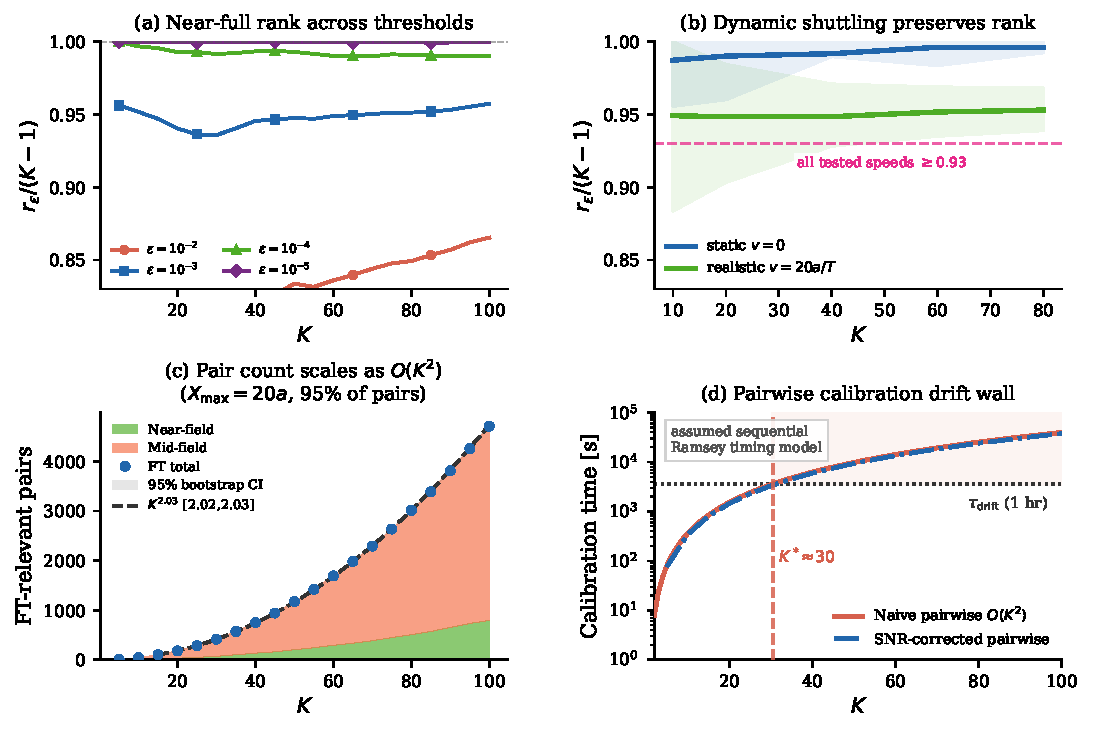
\includegraphics[width=\textwidth]{fig_summary.pdf}
\caption{\textbf{$O(K^2)$ calibration bottleneck for parallel spin-shuttling arrays.}
All results are evaluated on an $18\times18$ lattice ($a\sim100$\,nm) using the Stage~1 transport parameters ($v=20a/T$, $X_{\max}=20a$). Shaded bands denote one standard deviation over $N_{\rm trials}=30$ random spatial realizations unless otherwise stated.
(a) Normalized effective rank $r_\varepsilon/(K-1)$ of the gauge-projected susceptibility matrix versus active-qubit number $K$ for four relative thresholds $\varepsilon$. The matrix remains near-full-rank across the explored range.
(b) Comparison between the static geometry ($v=0$) and the realistic dynamic shuttling regime ($v=20a/T$), evaluated at $\varepsilon=10^{-3}$. Trajectory averaging changes the matrix entries but preserves the dense rank structure, with all tested speeds satisfying $r_\varepsilon/(K-1)\gtrsim0.93$.
(c) Number of fault-tolerant-relevant pairs ($|M_{ij}|>M_{\rm cut}$ with $\varepsilon_{\rm FT}=10^{-3}$), decomposed into near-field ($\mathrm{SNR}\ge3$) and mid-field ($\mathrm{SNR}<3$) components. The dashed curve shows a power-law fit $N_{\rm FT}\propto K^b$ with a bootstrap 95\% confidence interval for $b$, confirming quadratic growth over roughly $95\%$ of all possible pairs.
(d) Estimated calibration time versus $K$ under the assumed sequential pairwise Ramsey timing model. The naive pairwise protocol crosses the representative stability window $\tau_{\rm drift}=3600$\,s near $K^*\approx30$, whereas this panel should be read as a timing-model reference rather than a device-specific prediction.
}
\label{fig:summary}
\end{figure*}


\subsection{Numerical Validation of the Experimental Bottleneck}
\label{sec:numerical_bottleneck}

Our numerical analysis directly confirms the severity of this structural bottleneck. At precision thresholds relevant for fault-tolerant quantum logic ($\varepsilon_{\rm FT}\le10^{-3}$), the effective time-averaged susceptibility matrix remains near-full-rank across the explored system sizes (Fig.~\ref{fig:summary}a). The endpoint comparison between the static geometry and the realistic dynamic shuttling regime further shows that trajectory averaging modifies the matrix entries without collapsing the rank structure (Fig.~\ref{fig:summary}b). Thus, the parameter space does not trivially reduce to a low-dimensional manifold under the modeled shuttling dynamics.

We next evaluate the bottleneck in absolute physical units. For the adopted transport scale ($X_{\max}=20a$ and $U_J=X_{\max}T/2$), the number of couplings above the fault-tolerant relevance threshold grows quadratically with $K$ (Fig.~\ref{fig:summary}c). The fitted exponent is reported with a bootstrap confidence interval in the figure source data, rather than as an exact universal exponent; its role is to demonstrate that the relevant pair count remains consistent with $O(K^2)$ scaling in the simulated geometry.

The near-field/mid-field decomposition in Fig.~\ref{fig:summary}c separates pairs that are already well resolved at the baseline shot budget from weaker but still fault-tolerant-relevant pairs. This decomposition shows that the dominant obstacle is not a single poorly resolved coupling, but the large number of relevant matrix elements that must be experimentally characterized. Consequently, even if individual pair estimates are technically feasible, exhaustive sequential characterization remains structurally expensive.

Under the assumed sequential pairwise Ramsey timing model, this cost reaches the representative stability window $\tau_{\rm drift}=3600$\,s at a critical scale of order $K^*\approx30$ (Fig.~\ref{fig:summary}d). This number is not intended as a device-specific limit; it is a reference scale illustrating how a dense $O(K^2)$ calibration task can collide with finite parameter-stability times. The result motivates the multiplexed inference framework developed below, in which randomized parallel probing estimates the same dense susceptibility operator using $O(K)$ Ramsey rounds under idealized parallel readout.

\section{Structuring Phase Accumulation in Mobile Spin Architectures}
\label{sec:structured_phase}

The $O(K^2)$ dimensionality burden highlighted in Sec.~\ref{sec:calibration_bottleneck} and quantified in Sec.~\ref{sec:numerical_bottleneck} indicates that scalable spin shuttling cannot rely only on independent local phase calibration. It motivates a hardware-software co-design approach: the hardware should bound local phase dispersion and support multiplexed data acquisition, while the software compiler uses the inferred susceptibility model to track and compensate the residual macroscopic phase network.

\subsection{Bounding Phase Dispersion via Periodic Nanomagnets}
\label{sec:periodic_magnets}

To achieve the necessary hardware-level structuring, we exploit the periodic physical structure of the nanomagnet array originally designed for shuttling \cite{unseld_baseband_2025}. As established in Sec.~\ref{sec:phase_dynamics}, the local self-phase $\Delta\theta_i^{\text{self}}(T)$ absorbs independent single-qubit effects such as Stark shifts and static impurities. Because these local electrical contributions can be independently calibrated and tracked for each qubit, they do not uncontrollably accumulate through the transport geometry itself. Consequently, a dominant source of spatially extended phase dispersion during transport arises from the magnetic landscape.

By engineering the array to produce a spatially periodic magnetic field $B(x) = B_0 + \Delta B f(kx)$ with a magnetic spatial period $\lambda = 2\pi/k$, we can structurally bound this dispersion. We assume the spatial modulation $f(x)$ is a periodic function with a zero spatial average over one complete magnetic period, i.e., $\int_0^\lambda f(x) dx = 0$. In the rotating frame, the motion-induced magnetic phase ripple accumulated by an isolated qubit is governed by:
\begin{equation}
    \Delta\theta_i^{\text{ripple}}(T) = \gamma \Delta B \int_0^T f(k x_i(t)) dt.
    \label{eq:ideal_phase_ripple}
\end{equation}

If the qubit is shuttled at a constant velocity $v$ (such that $x_i(t) = vt$ and $dt = dx_i/v$) over exactly an integer number $q$ of magnetic periods, the spatial integral $\int_0^{q\lambda} f(x) dx$ vanishes, yielding $\Delta\theta_i^{\text{ripple}}(T) = 0$. Under realistic time-dependent velocity profiles $v_i(t)$, this perfect cancellation degrades because the temporal integration weights the spatial field non-uniformly. Nevertheless, a conservative bound follows directly from $|f(x)| \le \max|f(x)|$, ensuring that the magnetic phase ripple remains deterministically bounded by $|\Delta\theta_i^{\text{ripple}}| \le \gamma \Delta B T \max|f(x)|$.

Combined with the independently calibratable local offsets, the total local dispersion $\Delta\theta_i^{\text{self}}(T)$ remains constrained by the hardware periodicity and transit time. This highlights the true architectural role of the periodic nanomagnets: they act as a spatial filtering structure that constrains the accumulation of transport-induced phase dispersion, converting trajectory uncertainty into a bounded geometric functional.

\subsection{Relative Phase Tracking under Correlated Crosstalk}
\label{sec:coupled_tracking}

While Eq.~\eqref{eq:ideal_phase_ripple} guarantees a bounded local phase for an isolated qubit, the persistent correlated crosstalk disrupts this ideal behavior in a dense multi-qubit processor. As established in Sec.~\ref{sec:phase_dynamics} and Sec.~\ref{sec:calibration_bottleneck}, the deterministic component of the accumulated phase error during any given transport block is well characterized by the linear algebraic mapping $\boldsymbol{\Delta\theta} \approx \boldsymbol{\Delta\theta}^{\text{self}} + \mathbf{M} \mathbf{u}$. 

Because our physical framework explicitly separates transport-induced dispersion from stationary gate errors and stochastic noise, and structurally bounds local phase dispersion via the periodic nanomagnet array (Sec.~\ref{sec:periodic_magnets}), the control objective is not to physically force the macroscopic crosstalk to zero via increasingly stringent hardware isolation. Instead, the goal is to precisely evaluate this deterministic matrix-vector product for all active qubits.

Provided that a scalable and accurate model of the integrated susceptibility operator $\mathbf{M}$ is available—facilitated by the physics-informed structural parameterization introduced in Sec.~\ref{sec:learning}—this compensation reduces to a computationally tractable tracking problem. The evaluated relative errors can then be deterministically compensated via software-tracked virtual Z-gates ($R_z(-\Delta\theta_i)$) applied at the compilation level, which correspond to classical phase updates in the control frame rather than physical microwave pulses. This effectively rotates the computational frame to absorb the transport-induced dispersion without incurring additional physical gate or execution time overhead.

\subsection{Limitations of Analytical Control under Operational Constraints}
\label{sec:analytical_limits}

Given a reconstructed susceptibility model, forward phase evaluation is straightforward. Actively reshaping trajectories is more constrained because effective displacements must remain within adiabatic hardware bounds and close to the nominal routing schedule. The role of the inferred surrogate is therefore to move this refinement offline: once $\hat{\mathbf M}$ is reconstructed, bounded trajectory adjustments can be tested computationally under the same phase-dispersion objective. In the linearized model studied here, this refinement is optional; virtual-Z tracking remains the primary compensation mechanism used in the main scalability analysis.

\subsection{Architectural Implications for Scalable Spin-Shuttling Arrays}
\label{sec:architectural_implications}

The emergence of structured but analytically complex crosstalk necessitates a paradigm shift in how we define the fidelity of mobile qubit architectures. Traditionally, the fidelity of a quantum processor is decomposed into gate, readout, and routing components. However, our analysis reveals that \textit{phase compensation fidelity} constitutes a distinct limiting factor.

Under the assumption of independent and approximately Markovian error channels—a standard approximation in quantum noise modeling \cite{nielsen_quantum_2012}—we propose that the total system fidelity $F_{\text{total}}$ can be phenomenologically factorized to leading order as:
\begin{equation}
    F_{\text{total}} \approx F_{\text{gate}} \cdot F_{\text{transport}} \cdot F_{\text{comp}}.
    \label{eq:fidelity_decomposition}
\end{equation}
While the crosstalk-induced phase errors are intrinsically correlated across the qubit register, this factorization is justified as a leading-order phenomenological separation of error channels. Here, $F_{\text{comp}}$ captures the dominant correlated contribution that is not accounted for in conventional gate and transport fidelities, effectively measuring the overlap between the ideally phase-aligned state and the state subject to residual phase dispersion after software-based compensation. Similar to analytical decouplings commonly adopted in scalable shuttling-based architectures \cite{pino_demonstration_2021, langrock_blueprint_2023}, this decomposition should be interpreted as a practical metric rather than an exact composition identity for a completely positive trace-preserving (CPTP) channel composition identity.

Unlike $F_{\text{transport}}$, which addresses physical particle loss, non-adiabatic orbital excitations, or other transport-induced leakage processes (e.g., spin-orbit-induced spin flips or valley leakage), $F_{\text{comp}}$ isolates the correlated phase stability of the logical information encoded in the spin ensemble. As demonstrated in Sec.~\ref{sec:numerical_bottleneck}, in the absence of an active compensation framework, the macroscopic $O(K^2)$ phase network rapidly degrades $F_{\text{comp}}$ with increasing parallel operations. This imposes a practical calibration scalability bottleneck even if individual static gates ($F_{\text{gate}}$) are perfect and particles are transported safely.

Therefore, we treat deterministic relative phase compensation as an architectural control primitive for mobile spin platforms. The relevant bottleneck is not the nominal number of entries in $\mathbf{M}$ alone, but the wall-clock cost of learning a dense correlated phase network before low-frequency device drift changes the operating point. The framework developed below addresses this bottleneck by using multiplexed probing to acquire many linear constraints per Ramsey round and by applying software-level virtual-Z corrections from the inferred surrogate. The $1/r^3$ structural prior is used to organize the recovered matrix into a geometric baseline and a residual component; in the overdetermined regimes emphasized here, the observed scaling reduction originates from the multiplexed acquisition protocol rather than from a separate statistical advantage of the prior.

\section{Crosstalk Characterization and Scalable Calibration}
\label{sec:learning}

The structural bounds derived in Sec.~\ref{sec:structured_phase} establish that the susceptibility matrix $\mathbf{M}$ contains a dense $O(K^2)$ network of correlated phase responses. The goal of the calibration protocol is therefore not to make this operator sparse, but to learn it with fewer wall-clock calibration rounds than an exhaustive pairwise protocol would require.
By applying randomized multiplexed probes and reading out the register response in parallel, each Ramsey round supplies a full linear constraint on the dense phase network (Fig.~\ref{fig:figure1}c). The inferred surrogate then supports compiler-level virtual-Z compensation. The physics-informed $1/r^3$ baseline is retained as an interpretable coordinate system for the recovered matrix, separating the geometry-dominated component from residual device-specific disorder without claiming an independent reduction in the nominal $O(K^2)$ number of parameters.

\subsection{Multiplexed Inference and Statistical Limitations}
\label{sec:multiplexed_inference}

We model the deterministic crosstalk induced by simultaneous shuttling as a linear response between applied displacement controls and accumulated qubit phase shifts. For $K$ active qubits, the measured Ramsey phase-response vector $\Delta\boldsymbol\theta \in \mathbb{R}^K$ is written as:
\begin{equation}
    \Delta\boldsymbol\theta = \mathbf{M} \mathbf{u} + \boldsymbol{\epsilon},
\end{equation}
where $\mathbf{u} \in \mathbb{R}^K$ is the applied displacement vector, $\mathbf{M} \in \mathbb{R}^{K \times K}$ is the time-averaged dense crosstalk matrix, and $\boldsymbol{\epsilon}$ captures measurement noise and residual stochastic effects. We assume that deterministic local self-phases ($\Delta\theta_i^{\text{self}}$) are independently calibrated via single-qubit baseline transport and subtracted from the raw Ramsey data, up to residual calibration uncertainty absorbed into $\boldsymbol{\epsilon}$, thereby isolating the coupled crosstalk response as derived in Eq.~\eqref{eq:driven_phase} of Sec.~\ref{sec:phase_dynamics}.

State-of-the-art platforms have demonstrated limited forms of frequency-multiplexed dispersive readout across small qubit subsets \cite{philips_universal_2022, ruffino_cryo-cmos_2022}, providing an initial pathway toward parallel acquisition. However, in the context of this work, multiplexed probing refers generically to the application of parallel, independently addressable control signals and the simultaneous acquisition of qubit responses. This generic framework does not rely on a specific hardware implementation such as RF frequency multiplexing; rather, it can be realized through various modalities—including spatial parallelism, time-division batching, or frequency-domain addressing—depending on specific platform constraints. 

By applying randomized, independent displacement probes simultaneously to all active qubits---where each calibration displacement is drawn independently as $u_j \sim \mathcal{N}(0,U_J^2)$---and stacking $n_{\text{exp}}$ experimental configurations, we use the row-stacked data matrix convention implemented in the simulations:
\begin{equation}
    \mathbf{D}_{\theta} = \mathbf{U}\mathbf{M}^{T} + \mathbf{E},
\end{equation}
where the data matrix $\mathbf{D}_{\theta} \in \mathbb{R}^{n_{\text{exp}} \times K}$ collects one measured phase-response vector per row and $\mathbf{U} \in \mathbb{R}^{n_{\text{exp}} \times K}$ is the applied random probe matrix. The additive noise matrix $\mathbf{E}$ models the quantum projection noise, where each element $E_{ij}$ is independently drawn from a zero-mean Gaussian distribution with variance $\sigma_\varphi^2$. In this formulation, $\sigma_\varphi = 1/\sqrt{N_{\text{shots}}}$ denotes the projection-noise scale defined by the measurement shot budget.
Here, $n_{\text{exp}}$ denotes the number of distinct random displacement configurations (probe circuits). Each multiplexed experiment provides a global linear response of all qubits to a given randomized probe. 

We emphasize that this multiplexed probing is an offline system identification protocol, executed independently from the continuous, asynchronous operations of user-defined quantum algorithms. During this dedicated calibration phase, the phase acquisition is performed end-to-end via standard Ramsey interferometry. The active qubits are initialized in a superposition state while stationary, subjected to the randomized shuttling protocol $\mathbf{U}$ during which the correlated phases accrue, and subsequently read out simultaneously once parked at their respective measurement zones. 

This decouples phase accumulation from the readout mechanism, allowing for the simultaneous measurement of stationary qubits regardless of the complex kinematic reordering during transport. Once the macroscopic susceptibility surrogate $\hat{\mathbf{M}}$ is reconstructed from this offline procedure, the system returns to online execution. During actual quantum logic operations, phase dispersion is tracked and compensated entirely in software via virtual Z-gates without requiring any mid-circuit measurements.

Importantly, the reduction in experimental rounds arises because each randomized probe produces a vector-valued response from all $K$ active qubits. Each Ramsey round therefore supplies $K$ simultaneous linear constraints on the dense susceptibility matrix. The physical structure of the device is used to interpret the recovered operator as a geometry-dominated baseline plus a residual correction; it is not the primary reason that the round count scales linearly in the full-multiplexing regime.

While the number of required experimental configurations is dramatically reduced to $O(K)$, extracting the true expectation phases from realistic hardware requires averaging over quantum projection noise ($\mathbf{E}$). Each configuration must be averaged over standard projection shots (typically $N_{\text{shots}} \sim 10^3$). Therefore, the total acquisition time scales as:
\begin{equation}
    T_{\text{total}} \sim n_{\text{exp}} \cdot N_{\text{shots}} \cdot t_{\text{shot}},
\end{equation}
where $t_{\text{shot}}$ is the duration of a single measurement sequence. 

In the ideal noiseless limit ($\mathbf{E}=\mathbf{0}$), evaluating exactly $n_{\text{exp}} = K$ linearly independent probe configurations yields an exactly determined system, $\mathbf{M}^{T} = \mathbf{U}^{-1}\mathbf{D}_{\theta}$. However, this exact identifiability is a purely algebraic result that does not imply practical reconstructibility in realistic hardware. In practice, the naive full-matrix reconstruction of $\mathbf{M}$ is limited by the interplay between quantum projection noise ($\mathbf{E}$) and the conditioning of the probe matrix $\mathbf{U}$.

For a direct linear inversion, the estimation error is amplified by the inverse of the smallest singular value of the probe matrix, scaling as $\|\delta \mathbf{M}\| \lesssim \sigma_{\min}^{-1}(\mathbf{U}) \, \|\mathbf{E}\|$. In the general overdetermined regime ($n_{\text{exp}} > K$), this inversion is formally executed via the Moore-Penrose pseudo-inverse $\mathbf{U}^+$. Equivalently, this implies a strong dependence on the condition number $\kappa(\mathbf{U})$, such that poorly conditioned designs lead to significant noise amplification. When $n_{\text{exp}}$ is only marginally larger than $K$, random probe matrices become poorly conditioned with high probability, as the smallest singular value becomes arbitrarily small in this near-square regime \cite{vershynin_high-dimensional_2018}. This leads to noise amplification during inversion, rendering the minimal algebraic requirement $n_{\text{exp}} = K$ practically insufficient.

In particular, well-conditioned linear regression typically requires an oversampling ratio $n_{\text{exp}}/K$ bounded away from unity to control estimator variance \cite{hastie_elements_2009}. This implies that stable estimation requires a non-negligible oversampling factor, i.e., $n_{\text{exp}} = cK$ with $c > 1$ sufficiently bounded away from unity. However, enforcing such well-conditioned designs under experimental constraints is nontrivial, and typically leads to a larger constant-factor overhead within the linear-scaling regime.

Near the algebraic limit, conditioning rather than rank alone controls the practical estimator variance. In the simulations below, a moderately overdetermined budget ($n_{\text{exp}}=2K$) is used as the main operating point because it is empirically sufficient to stabilize the randomized probe matrix under the adopted shot-noise model. The crucial scaling point is that this budget remains linear in $K$, whereas pairwise calibration requires $K(K-1)/2$ sequential interrogations.

While this parallel acquisition theoretically compresses the experimental scaling, we acknowledge the practical hardware constraints of near-term cryogenic platforms. Implementing simultaneous parallel control across a massive dense array ($K \gg 10$) faces platform-specific bottlenecks, including wiring density, frequency crowding, and thermal dissipation limits \cite{vandersypen_interfacing_2017, gonzalez-zalba_scaling_2021, bartee_spin-qubit_2025}. However, the proposed architecture is directly compatible with block-structured control architectures, such as crossbar addressing schemes \cite{veldhorst_silicon_2017, li_crossbar_2018}, which naturally enforce sub-array level parallelism where subsets of $m$ qubits are driven simultaneously. This practical constraint increases the required experimental overhead. In the sub-array protocol studied below, the calibration time remains $T_{\rm cal}=n_{\rm exp}T_{\rm Ramsey}$, with the required overhead $n_{\rm exp}/K$ increasing as the multiplexing capacity $m$ decreases; this still preserves a structural advantage over exhaustive pairwise calibration. Our subsequent numerical results therefore represent the scaling achievable under idealized parallel probing conditions, serving as a reference scaling limit for the proposed inference framework.

\subsection{Physics-Informed Structural Reduction}
\label{sec:physics_inference}

To make the recovered dense operator physically interpretable, we partition the dynamic susceptibility matrix into a static geometric baseline and a dynamically driven residual, $\mathbf{M} = \mathbf M_{\rm prior} + \Delta\mathbf M_{\rm res}$. The static matrix $\mathbf M_{\rm prior}$ captures the leading geometry-derived spatial decay, approximated here by a dipole-like $\sim 1/r^3$ response evaluated at the nominal parking coordinates. The calibration can then be written as a residual regression around this baseline. From the multiplexed observational data, we form
\begin{equation}
    \mathbf{D}_{\rm res} = \mathbf{D}_{\theta} - \mathbf U\mathbf M_{\rm prior}^{T},
\end{equation}
and reconstruct the residual operator $\Delta\mathbf M_{\rm res}$ via least-squares estimation. 

This decomposition should not be interpreted as the origin of the $O(K)$ experimental scaling in the overdetermined setting used for the main figures. When the same well-conditioned probe matrix is used, residual regression around $\mathbf M_{\rm prior}$ and plain multiplexed least squares produce the same estimator up to numerical precision. Its role is instead interpretive: it separates the macroscopic geometric baseline from the residual device-specific correction, which makes the inferred susceptibility network easier to audit, compare across devices, and use as a physically grounded surrogate for optional control refinement.

\subsection{Surrogate-Assisted Trajectory Optimization}
\label{sec:trajectory_optimization}

Once the predictive surrogate $\hat{\mathbf{M}}$ is reconstructed, the inverse problem of actively shaping transport trajectories $\mathbf{u}$ is executed computationally. The optimization algorithm targets the minimization of the relative phase dispersion across the active register, defined as the projected relative phase variance:
\begin{equation}
    \mathcal{L}(\mathbf{u}) = \|\mathbf{P} \hat{\mathbf{M}} \mathbf{u}\|^2 + \lambda \|\mathbf{u} - \mathbf{u}_{\text{nom}}\|^2,
\end{equation}
where $\mathbf{P} = \mathbf{I} - \frac{1}{K}\mathbf{1}\mathbf{1}^\top$ is the projection matrix introduced in Sec.~\ref{sec:calibration_bottleneck}. This projection operator removes the global phase degree of freedom, ensuring that the optimization only targets physically relevant relative phase errors.
Here, the column vector $\mathbf{u} \in \mathbb{R}^K$ collects the time-integrated shuttling displacements $u_j$ of all active qubits. The regularizer $\lambda$ penalizes large deviations from the nominal displacement $\mathbf{u}_{\text{nom}}$ (the baseline macroscopic routing schedule dictated by the quantum compiler). To ensure adherence to adiabatic hardware limits, these kinematic variables are bounded by physical constraints, $u_j \in [U_{\min}, U_{\max}]$.

The objective function is quadratic in $\mathbf{u}$ with a positive semidefinite Hessian given by $2(\hat{\mathbf{M}}^\top \mathbf{P} \hat{\mathbf{M}} + \lambda \mathbf{I})$, guaranteeing convexity in the linearized model. We use this surrogate optimization as a consistency check showing that the reconstructed operator can be inserted into a constrained control objective without additional hardware queries. It is not the primary scalability mechanism: the main compensation protocol is software-level virtual-Z tracking using the reconstructed susceptibility matrix.

The analytical gradient and Hessian structure required for efficient numerical optimization are detailed in Appendix~\ref{app:extended_analysis}. Under the linearized phase model introduced in Sec.~\ref{sec:calibration_bottleneck}, the constrained L-BFGS-B solver converges reliably within the feasible displacement bounds. The appendix reports both the surrogate objective evaluated on $\hat{\mathbf{M}}$ and the physical phase variance evaluated on the true simulation matrix, explicitly distinguishing trajectory phase dispersion from the reconstruction-residual fidelity $F_{\rm comp}$.

\begin{figure*}[t!]
\centering
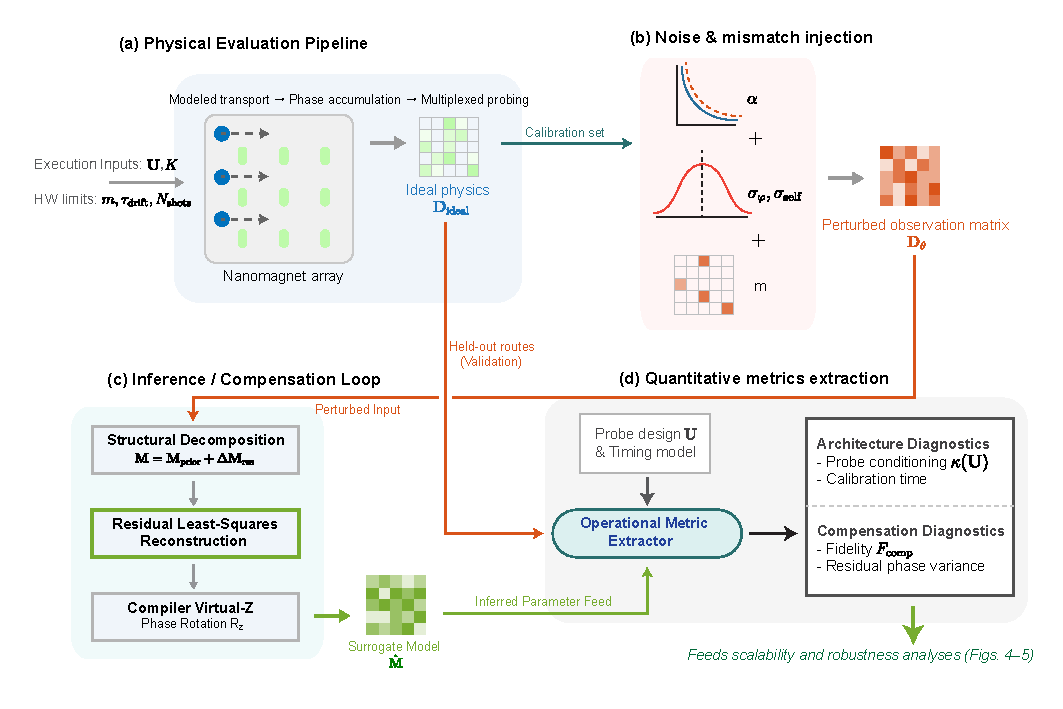
\includegraphics[width=\textwidth]{fig_operational_validation_lifecycle.pdf}
\caption{\textbf{Operational validation framework and deployment lifecycle for correlated phase tracking.}
(a) Physical evaluation pipeline. The execution stage is initialized by a set of routing or calibration probes $\mathbf U$, the active register size $K$, and hardware-level constraints including the finite multiplexing capacity $m$, the drift time $\tau_{\rm drift}$, and the shot budget $N_{\rm shots}$. Within the adopted transport model, the nanomagnet-induced spatial frequency landscape maps parallel shuttling trajectories into an ideal phase-response matrix $\mathbf D_{\rm ideal}$, representing the deterministic transport-induced phase response before measurement noise and bandwidth constraints are applied.
(b) Noise, mismatch, and bandwidth injection. To test operational robustness, the ideal response is perturbed by structural prior mismatch $\alpha$, projection noise $\sigma_\varphi$, residual self-phase noise $\sigma_{\rm self}$, and a finite sub-array probing mask with at most $m$ nonzero input displacements per calibration round. This produces the measured response matrix $\mathbf D_\theta$, separating the deterministic susceptibility structure from stochastic residuals and finite-bandwidth sampling effects.
(c) Inference and software compensation loop. The measured response matrix $\mathbf D_\theta$ is processed by an offline system-identification pipeline. A physics-informed baseline--residual decomposition,
$\mathbf M=\mathbf M_{\rm prior}+\Delta\mathbf M_{\rm res}$, separates the geometric $1/r^3$ reference susceptibility from device-specific residual corrections. Residual least-squares reconstruction then yields a surrogate susceptibility matrix $\hat{\mathbf M}$, which is used by the compiler to map inferred phase corrections into virtual-$Z$ frame updates $R_z$, without requiring additional physical compensation gates.
(d) Quantitative validation and metric extraction. The reconstructed surrogate $\hat{\mathbf M}$ is evaluated on held-out routing or probe configurations together with the corresponding probe design $\mathbf U$ and the assumed timing model. The validation layer extracts the compensation fidelity $F_{\rm comp}$, probe-conditioning metric $\kappa(\mathbf U)$, calibration time $T_{\rm cal}$, and residual gauge-projected phase variance. These quantities provide the operational link between the inference pipeline and the scaling and robustness analyses reported in the following figures.}
\label{fig:operational_framework}
\end{figure*}

\section{Numerical Demonstration and Scalability Analysis}
\label{sec:simulation_results}

To quantitatively validate the proposed hardware-software co-design framework, we perform numerical simulations of a dense two-dimensional spin-shuttling array using the normalized model and cost assumptions specified in Methods. The simulations are designed to test a structural claim: a dense correlated phase network that would require $O(K^2)$ pairwise calibration can be identified and compensated using $O(K)$ multiplexed Ramsey rounds under idealized parallel probing.
Within this model, the working point $n_{\text{exp}}=2K$ maintains high compensation fidelity across the explored range, while the corresponding pairwise protocol crosses the assumed drift-time window near $K\approx 30$. These numerical thresholds should be read as reference scaling limits under the stated noise and timing assumptions, not as device-specific performance guarantees.


\begin{figure*}[t]
\centering
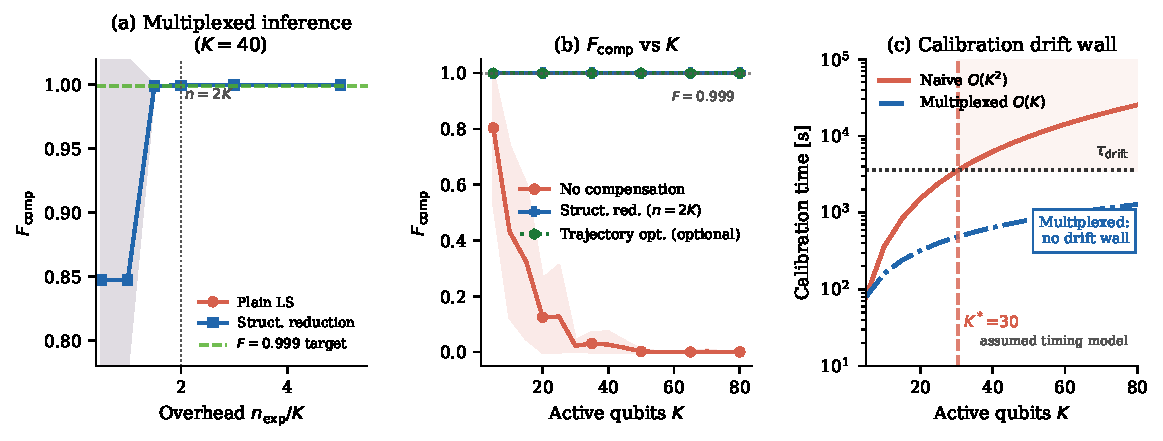
\includegraphics[width=\textwidth]{fig_2_summary.pdf}
\caption{\textbf{Scalable phase compensation via multiplexed inference and virtual Z-gates.}
All simulations use an $18\times18$ lattice ($a\approx100$~nm) with the Stage-1 transport parameters ($v=20a/T$, $X_{\rm max}=20a$).
(a) Compensation fidelity $F_{\rm comp}$ versus calibration overhead $n_{\rm exp}/K$ at $K=40$. Plain multiplexed least squares (red) and the $1/r^3$ structural decomposition (blue) reach the target regime at the same overdetermined budget, $n_{\rm exp}=2K$, because the same well-conditioned probe data determine both estimators. This overlap is an intended ablation: the experimental scaling reduction originates from multiplexed probing, while the structural prior supplies an interpretable baseline--residual decomposition.
(b) $F_{\rm comp}$ versus active qubits $K$ under independent randomized routing displacements $u_j\sim\mathcal{U}[-U_J,U_J]$. Without compensation (red), coherent crosstalk accumulation rapidly suppresses the phase-alignment fidelity. Virtual-Z compensation using the reconstructed surrogate (blue) maintains high fidelity across the simulated range; surrogate trajectory optimization (green) is shown only as an optional refinement and is not required for the nominal linear model.
(c) Calibration time versus $K$ under the assumed sequential timing model. Pairwise interrogation scales as $O(K^2)$ and crosses the representative drift window near $K^*\approx30$, whereas the multiplexed protocol uses $n_{\rm exp}=2K$ Ramsey rounds and remains within the window for all simulated $K$.}
\label{fig:summary2}
\end{figure*}

\subsection{Empirical Scaling and Limitations of Uncompensated Routing}
\label{sec:naive_failure}

We first evaluate the scaling of the physical crosstalk network. We define functionally relevant crosstalk pairs by $|M_{ij}| > \varepsilon_{\text{FT}}/U_J$, corresponding to a maximum induced phase error above the reference threshold $\varepsilon_{\text{FT}}=10^{-3}$ under the characteristic displacement scale $U_J$. As shown in Sec.~\ref{sec:numerical_bottleneck}, the number of non-negligible crosstalk pairs scales approximately quadratically with $K$ in the adopted reference model, producing the calibration bottleneck targeted by multiplexed probing; the corresponding ideal response-generation stage is sketched in Fig.~\ref{fig:operational_framework}(a).

In the absence of active compensation—meaning the compiler applies zero virtual Z-gate corrections, effectively operating under the assumption of a null surrogate $\hat{\mathbf{M}} = \mathbf{0}$—the unmitigated crosstalk induces a relative phase variance that scales at least linearly with $K$ in expectation ($\text{Var}_{\text{rel}} \propto K$), due to the dense summation over correlated crosstalk contributions under independent random displacements with finite variance. Assuming approximately Gaussian-distributed phase fluctuations, the compensation fidelity decays exponentially with this relative variance ($F_{\text{comp}} \approx \exp(-\text{Var}_{\text{rel}}/2)$), causing a rapid collapse of fidelity to near-zero values for $K \gtrsim 20$. As shown by the uncompensated baseline (red curve) in Fig.~\ref{fig:summary2}(b), this collapse persists even under a randomized routing schedule ($u_j \sim \mathcal{U}[-U_J, U_J]$).

Plain multiplexed least-squares regression already exposes the central statistical feature of the problem. Near the algebraic identifiability limit ($n_{\text{exp}}=K$), random probe matrices are often ill-conditioned, so finite shot noise is amplified by the pseudo-inverse; this probe-conditioning diagnostic is one of the validation outputs summarized in Fig.~\ref{fig:operational_framework}(d). At the moderately overdetermined working point used throughout the main text ($n_{\text{exp}}=2K$), the same randomized design becomes sufficiently stable to support high-fidelity compensation in the adopted simulation model.
This behavior clarifies the role of the structural prior. It is not needed to explain the observed $O(K)$ round scaling under full multiplexing; instead, it provides a physically meaningful decomposition of the recovered operator, which is useful for interpretation, diagnostics, and future extensions to more bandwidth-limited or ill-conditioned regimes.

\subsection{Scalable Phase Compensation via Virtual Z-Gates}
\label{sec:structured_recovery}

To properly contextualize this scalable inference, we apply the structured framework derived in Sec.~\ref{sec:physics_inference}, whose baseline--residual reconstruction and virtual-$Z$ compensation path are summarized in Fig.~\ref{fig:operational_framework}(c). A useful observation from our simulations is that subtracting the geometric prior ($\mathbf M_{\rm prior}$) does not significantly reduce the Frobenius norm of the parameter space ($||\Delta\mathbf{M}_{\text{res}}||_F / ||\mathbf{M}_{\text{prior}}||_F \approx 1.23$). 

Consequently, as illustrated in Fig.~\ref{fig:summary2}(a), the structured regression (blue curve) and the plain multiplexed LS (red curve) exhibit the same $F_{\text{comp}}$ trajectory under the same probe matrix $\mathbf{U}$, reaching the target regime at $n_{\text{exp}}=2K$. This agreement is a useful ablation rather than a weakness: it shows that, in the overdetermined full-multiplexing regime, the measurement data determine the estimator and the scaling advantage is primarily due to multiplexed probing.
The structural prior remains useful because it assigns the recovered dense matrix a physical coordinate system. It separates the geometry-dominated $1/r^3$ baseline from residual device-specific disorder and thereby makes the inferred surrogate auditable without overstating a statistical regularization effect in the main operating regime.

The macroscopic compensation fidelity is supported by microscopic reconstruction accuracy. The element-wise analysis in Appendix~\ref{app:extended_analysis} shows that, at $K=40$ and $n_{\text{exp}}=2K$, the inferred susceptibility matrix closely tracks the simulated ground truth, including the near-field entries that dominate phase accumulation. Thus, the high $F_{\text{comp}}$ values are not merely a consequence of fitting a single macroscopic metric; they reflect a consistent reconstruction of the dense interaction network under the stated model and noise assumptions.

Operating on the reconstructed surrogate $\hat{\mathbf{M}}$, the compiler applies virtual-Z corrections that remove the predicted deterministic relative phases. As shown in Fig.~\ref{fig:summary2}(b), this software-level tracking maintains high compensation fidelity up to $K=80$ in the normalized simulation model. The nearly overlapping trajectory-optimization curve indicates that, for the nominal linear model tested here, physical trajectory reshaping is not required to obtain the reported compensation performance. We therefore interpret the trajectory optimizer as an optional surrogate-consistency check, potentially relevant for future nonlinear or time-dependent error models rather than as the source of the main scalability result.

\begin{figure*}[t]
\centering
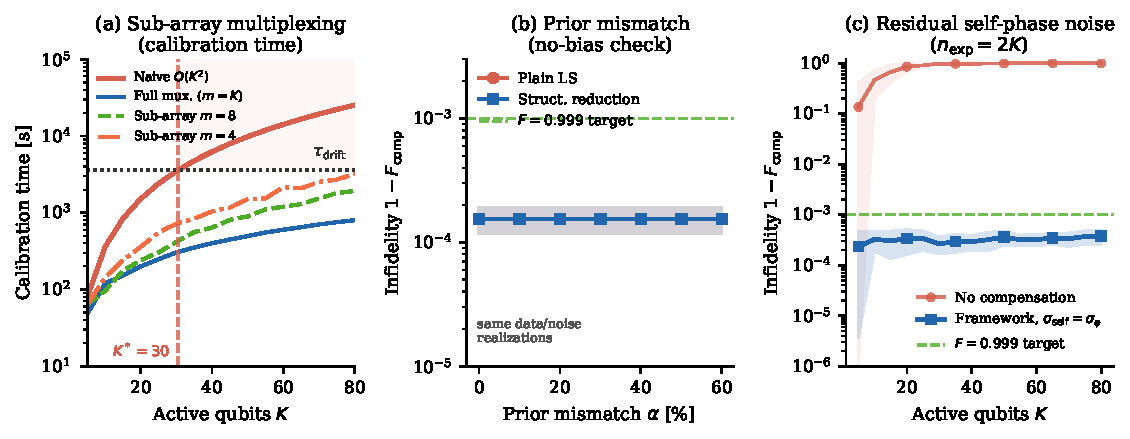
\includegraphics[width=\textwidth]{fig_3_robustness_summary.pdf}
\caption{\textbf{Robustness of multiplexed phase compensation under hardware constraints.}
All results use the same normalized $18\times18$ lattice model and matched random seeds for paired comparisons.
(a) Calibration time versus $K$ for naive pairwise interrogation and sub-array multiplexing capacities $m=K,8,4$. The plotted times use empirically determined minimum overheads to reach the target fidelity and should be interpreted under the assumed sequential Ramsey timing model.
(b) Prior-model mismatch displayed as infidelity $1-F_{\rm comp}$ for matched probe/noise realizations at $K=40$ and $n_{\rm exp}=2K$. The near-overlap of plain LS and structural reduction indicates that the overdetermined data, rather than the prior, determine the estimator in this regime.
(c) Residual self-phase noise displayed as infidelity $1-F_{\rm comp}$, with an uncompensated baseline included for scale. Active virtual-Z compensation suppresses deterministic crosstalk while the remaining error is set by the stochastic noise floor. Extended fidelity and overhead scans are provided in Appendix~\ref{app:robustness}.}
\label{fig:robustness_summary}
\end{figure*}

\subsection{Practical Scalability and Robustness under Hardware Constraints}
\label{sec:subarray_scaling}

While the preceding results demonstrate the framework within the adopted idealized parallel-probing model, near-term cryogenic platforms face wiring and readout bandwidth constraints. To address these key experimental constraints, we evaluate the calibration overhead under sub-array multiplexing protocols, where hardware limits the simultaneous probing capacity to $m$ qubits per experimental round; the corresponding finite-bandwidth and noise-injection layer is indicated in Fig.~\ref{fig:operational_framework}(b). 

Figure~\ref{fig:robustness_summary}(a) illustrates the total calibration time under limited parallel capacities ($m=4$ and $m=8$), which model finite control/readout bandwidth rather than a change in the underlying susceptibility network. Reducing $m$ increases the required number of randomized probe rounds, but the resulting time still remains far below exhaustive pairwise interrogation over much of the explored range. Under the assumed timing model, $m=8$ remains inside the representative drift window through $K=80$, while $m=4$ substantially extends the drift-limited scale relative to naive pairwise calibration.
The extended scans in Appendix~\ref{app:robustness} report both the fixed-budget fidelity at $n_{\text{exp}}=3K$ and the empirically determined minimum overhead $n_{\text{exp}}^*/K$. These results should be read as bandwidth-constrained reference simulations: they quantify how the multiplexed protocol degrades gracefully as parallel capacity is reduced, rather than hardware-specific timing predictions for a particular cryogenic implementation.

Beyond measurement bandwidth constraints, Fig.~\ref{fig:robustness_summary}(b,c) reports robustness in terms of infidelity rather than absolute $F_{\rm comp}$, making the small residual differences visible. The prior-mismatch experiment perturbs the true susceptibility away from the ideal $1/r^3$ baseline while evaluating plain LS and structural reduction on matched data. Their overlap is the expected behavior of an overdetermined least-squares estimator: the data-driven solution absorbs the mismatch when $\mathbf{U}$ is well-conditioned, so the prior does not introduce a detectable bias.

The residual self-phase-noise experiment separates deterministic crosstalk tracking from stochastic phase fluctuations. When stochastic self-phase noise is comparable to the projection-noise scale, active virtual-Z compensation still removes the deterministic network contribution, whereas the uncompensated baseline rapidly loses phase alignment. The remaining infidelity should therefore be interpreted as the residual noise floor of the adopted model, not as a claim of device-independent absolute fidelity.

\section{Conclusion and Outlook}
\label{sec:conclusion}

In this work, we have analyzed transport-induced correlated dephasing as a scalability bottleneck in dense spin-shuttling architectures. By reformulating shuttling-induced phase errors as a deterministic spatial susceptibility operator, we showed that relative-phase calibration can acquire an $O(K^2)$ dimensionality burden in dense parallel routing. Without compensation, this dense crosstalk network substantially degrades phase-alignment fidelity as the active register grows.

To address this bottleneck, we proposed a hardware-software framework in which multiplexed Ramsey probing is the primary mechanism that compresses the calibration round count from pairwise $O(K^2)$ interrogation to an $O(K)$ protocol. In the normalized simulations, the working point $n_{\text{exp}}=2K$ is sufficient for stable virtual-Z compensation under idealized parallel probing. The $1/r^3$ structural prior provides a physically interpretable baseline--residual decomposition of the recovered susceptibility matrix, but it is not the source of the scaling reduction in the overdetermined full-multiplexing regime. The multiplexing notion used here is implementation-agnostic and refers to parallel, independently addressable control and measurement operations rather than to a specific frequency-domain readout mechanism.

Operating on this surrogate, deterministic relative phases can be tracked at the software level through virtual-Z updates, substantially reducing the practical calibration burden without requiring physical trajectory modification in the nominal linear model. The numerical thresholds reported here---including the drift wall near $K\approx30$ for pairwise calibration and the high-fidelity compensation values---depend on the normalized coupling scale, shot-noise model, and simplified timing assumptions. They should therefore be interpreted as reference scaling limits for the modeled architecture, rather than exact device-specific predictions. 

Importantly, the $O(K^2)$ parameter bottleneck arises generically from the dense pairwise coupling structure intrinsic to long-range interactions, and is largely insensitive to the precise functional form of the coupling. Consequently, the validity of the $O(K)$ multiplexed inference framework itself does not depend on the specific choice of the dipolar model, but only on the existence of a structured, deterministic crosstalk network. The efficiency of this multiplexed inference protocol does not rely on reducing the nominal dimensionality of the parameter space, but rather on simultaneous vector-valued probing under the underlying physical interaction.

Looking forward, the framework developed here provides reference scaling limits under idealized parallel control and measurement assumptions. Near-term hardware may limit the available probe bandwidth to localized sub-arrays, making conditioning, drift, and re-calibration scheduling central practical questions. The present results therefore motivate, but do not yet replace, future device-level studies that combine bandwidth-constrained sensing, non-dipolar corrections, and measured noise spectra.

To address the limitations of the leading-order spatial model and move toward hardware-specific predictions, future investigations will integrate complete open-quantum-system dynamics and rigorous device-level physics. Specifically, we plan to employ detailed density-matrix simulations (e.g., via QuTiP) coupled with high-fidelity micromagnetic solvers (e.g., Ubermag) to accurately capture device-specific prefactors, angular anisotropies, and higher-order transverse spin mixing. Ultimately, by coupling this high-fidelity physical modeling with scalable data-driven control strategies, this framework lays the foundation for robust, automated control stacks in next-generation solid-state quantum architectures.

\section*{Methods: Numerical Simulation and Experimental Cost Model}

\subsection*{Physical Model and Lattice Dynamics}
All large-scale numerical simulations are conducted on a finite two-dimensional square lattice of size $18 \times 18$ with a normalized lattice constant $a=1$. This scale accommodates active qubit subsets $K \in [5,80]$, which are uniformly sampled without replacement while minimizing finite-size edge effects. Stage-1 rank and calibration-bottleneck scans use $N_{\text{trials}}=30$ realizations with bootstrap confidence intervals for the power-law fit; Stage-2 scaling and robustness scans use $N_{\text{trials}}=15$ realizations, with the fixed-$K$ inference-overhead panel evaluated over 30 trials. The vertical nanomagnet separation is modeled at $z=0.35a$. 

To capture the dominant coherent crosstalk, the dynamic time-averaged susceptibility matrix $\mathbf{M}$ is computed using a macroscopic transport distance of $X_{\max} = 20a$, with a fixed transit time $T_{\text{trans}} = 1.0$, defining the nominal displacement bound $U_J = X_{\max}T_{\text{trans}}/2$. We explicitly adopt a dipole-dominated susceptibility model ($\chi_{ij} \sim 1/r^3$), which captures the leading-order spatial structure of nanomagnet stray fields. While device-specific electrostatic prefactors and magnetic angular anisotropies will inevitably modify the exact quantitative magnitude of individual couplings, they do not qualitatively alter the leading scaling behavior or the dense connectivity arising from long-range dipolar interactions. 

Furthermore, to explicitly break artificial lattice symmetries and simulate operational disorder, we introduce uniformly distributed velocity fluctuations ($\pm 15\%$) and static positional disorder (up to $35\%$ of $a$). These conservative values reflect experimentally reported levels of charge disorder and control inhomogeneity in semiconductor quantum dot arrays \cite{yoneda_quantum-dot_2018, struck_low-frequency_2020}, serving to rigorously stress-test the robustness of the proposed framework.

\subsection*{Measurement Protocol and Noise Limits}
To model quantum projection noise, simulated expectation phases are subjected to Gaussian noise with standard deviation $\sigma_\varphi = 1/\sqrt{N_{\text{shots}}}$, assuming a baseline budget of $N_{\text{shots}} = 1000$ typical measurement repetitions per experimental configuration.
The cutoff magnitude for fault-tolerant relevance is defined as $M_{\mathrm{cut}} = \varepsilon_{\mathrm{FT}} / U_J$, where $\varepsilon_{\mathrm{FT}} = 10^{-3}$. Under the normalized simulation scale, the interaction density is extremely high, with approximately $95\%$ of all possible pairs nominally exceeding this threshold. However, we explicitly note that the effective observability of these long-range interactions is directly governed by the physical signal-to-noise ratio. In physical regimes where the device-specific prefactor $C_{\text{phys}}$ is small, weak long-range couplings may fall below the projection noise floor. This competition between signal magnitude and shot noise can lead to an effectively sparse observable matrix in practice, despite its formally dense algebraic structure. The single-entry uncertainty scales as $\sigma_M = \sigma_\varphi / U_J$; notably, the macroscopic $20a$ displacement generates sufficient signal magnitude to avert extreme measurement penalties for mid-field pairs.

For calibration timing, the duration of a single multiplexed Ramsey sequence is conservatively estimated at $t_{\text{shot}} = 8$\,ms, yielding an effective experimental round time of $T_{\text{Ramsey}} \approx 8$\,s under a simplified timing model. 

Under the bandwidth-constrained sub-array protocols ($m < K$), we do not hold the displacement configuration $\mathbf{u}$ constant to sequentially exhaust all $K$ readouts. Instead, we adopt a stochastic sub-sampled measurement protocol in which each experimental round employs a newly randomized transport configuration $\mathbf{u}$, from which only a randomly selected subset of $m$ qubits is probed. By leveraging the randomness of the multiplexed control matrix $\mathbf{U}$ to ensure robust parameter inversion, this partial observation model avoids the $K/m$ multiplicative overhead. This reduces the wall-clock calibration time to scale as $T_{\text{cal}} = n_{\text{exp}} \cdot T_{\text{Ramsey}}$, at the expense of requiring continuously randomized control configurations and relying on global regression for comprehensive matrix reconstruction.

We explicitly note that this protocol represents an optimistic lower bound on calibration time. It assumes negligible overhead from qubit re-initialization, shuttling latency, and classical control constraints. The reported temporal analysis, including the drift-limited stability window ($\tau_{\text{drift}} \approx 3600$\,s), should therefore be interpreted as a validation of the structural scaling properties of the multiplexed inference framework, rather than an exact, device-faithful temporal prediction.

\subsection*{Inference, Fidelity, and Scale Invariance}
To evaluate the compensation fidelity $F_{\text{comp}}$, we employ a realistic, randomized routing schedule where each qubit's nominal displacement is drawn independently from a uniform distribution, $u_j \sim \mathcal{U}[-U_J, U_J]$. This ensures the evaluation captures statistically typical operating conditions rather than adversarial or worst-case configurations. Fidelity is computed based on the residual relative phase variance after applying software-tracked virtual Z-gate corrections derived from the reconstructed surrogate $\hat{\mathbf{M}}$. All numerical routines and structural reductions were implemented using standard linear algebra libraries without imposing explicit sparsity constraints.

In our numerical models, the deterministic crosstalk matrix is computed using a normalized prefactor. Physically, the true susceptibility matrix scales as $\mathbf{M}_{\text{phys}} = C_{\text{phys}} \mathbf{M}_{\text{sim}}$, where the global scalar $C_{\text{phys}}$ depends on the specific device gyromagnetic ratio, dot spacing, and field gradient constraints. 
The identifiability of the inference problem depends on the rank and conditioning of the probe matrix $\mathbf{U}$. In the overdetermined regime ($n_{\text{exp}} > K$), the total susceptibility matrix is uniquely determined by the measurement data, provided that $\mathbf{U}$ has full column rank and is sufficiently well-conditioned. 

Under these conditions, the final compensation fidelity becomes largely insensitive to moderate global rescaling or local perturbations of the prior model, within the tested regime. This behavior reflects the intrinsic identifiability of the system rather than reliance on explicit numerical regularization, although conditioning effects remain relevant in the presence of finite noise. Consequently, the robustness of the framework is governed primarily by the information content of the multiplexed measurements, provided that sufficient oversampling (e.g., $n_{\text{exp}} \gtrsim 2K$) is achieved and a well-conditioned probe matrix is maintained.

However, we emphasize that the reported compensation fidelities ($F_{\text{comp}} > 0.999$) correspond to a normalized simulation regime. In physical systems, the absolute achievable fidelity relies on the direct interplay between the macroscopic prefactor $C_{\text{phys}}$ and the projection noise floor. Consequently, these numerical values should be interpreted as representative of the structurally achievable regime enabled by the multiplexed framework, rather than device-specific performance guarantees. Ultimately, our numerical evaluation is designed to validate the structural scaling trends and the algorithmic viability of the hardware-software co-design, rather than to serve as a device-faithful quantitative simulation.




\subsection*{Statistical Reporting and Reproducibility}
All numerical results are generated from deterministic Python scripts using explicitly seeded pseudo-random number generators. Stage-1 bottleneck and rank analyses use $N_{\rm trials}=30$ random active-register placements; the reported power-law exponent for the number of fault-tolerant-relevant pairs is accompanied by a non-parametric bootstrap confidence interval computed from $N_{\rm boot}=1000$ resamples. Stage-2 scaling and robustness scans use $N_{\rm trials}=15$ realizations, except for the fixed-$K$ inference-overhead panel, which uses 30 trials. Shaded bands in the figures denote one standard deviation over the stated ensembles unless otherwise specified.

The principal plotted quantities are generated as source-data CSV files by the accompanying scripts. The Stage-1 script outputs \path{source_data_stage1_rank_threshold.csv}, \path{source_data_stage1_rank_disorder.csv}, \path{source_data_stage1_speed.csv}, \path{source_data_stage1_FT_pairs.csv}, \path{source_data_stage1_powerlaw_fit.csv}, and \path{source_data_stage1_calibration_time.csv}. The Stage-2 inference script outputs \path{source_data_stage2_inference_overhead.csv}, \path{source_data_stage2_reconstruction_scatter.csv}, \path{source_data_stage2_trajectory_history.csv}, \path{source_data_stage2_trajectory_profile.csv}, \path{source_data_stage2_scaling.csv}, and \path{source_data_stage2_summary_scalars.csv}. The robustness script outputs \path{source_data_stage2_robustness_subarray_overhead.csv}, \path{source_data_stage2_robustness_subarray_F_at_3K.csv}, \path{source_data_stage2_robustness_prior_mismatch.csv}, and \path{source_data_stage2_robustness_selfphase_Kscan.csv}. These files contain the plotted means, standard deviations, fitted curves, and scalar diagnostic values needed to regenerate the main and extended numerical figures.


\begin{table*}[t!]
\centering
\caption{Default numerical configuration used in the simulations. Values are dimensionless unless a time unit is shown. These parameters define the normalized reference model and should not be interpreted as device-calibrated predictions for a specific chip.}
\label{tab:simulation_parameters}
\renewcommand{\arraystretch}{1.2}
\begin{tabular}{lll}
\hline
Quantity & Value & Role in the simulation \\
\hline
Lattice & $18\times18$ sites, $a=1$ & \makecell[l]{finite array from which active \\ subsets are sampled} \\
Active register & $K\in[5,80]$ & simultaneously shuttled qubits \\
Nanomagnet depth & $z=0.35a$ & regularizes the dipolar $1/r^3$ kernel \\
Transport scale & \makecell[l]{$X_{\max}=20a$, \\ $T_{\rm trans}=1$} & \makecell[l]{sets nominal displacement scale \\ $U_J=X_{\max}T_{\rm trans}/2$} \\
Velocity disorder & $\pm15\%$ & breaks artificial trajectory symmetry \\
Static positional disorder & up to $0.35a$ & stress test for lattice imperfections \\
Projection noise & $N_{\rm shots}=1000$, $\sigma_\varphi=1/\sqrt{N_{\rm shots}}$ & Ramsey phase readout noise \\
Single-entry uncertainty & $\sigma_M=\sigma_\varphi/U_J$ & \makecell[l]{measurement uncertainty of \\ inferred matrix entries} \\
FT relevance threshold & $\varepsilon_{\rm FT}=10^{-3}$, $M_{\rm cut}=\varepsilon_{\rm FT}/U_J$ & pairwise inclusion criterion in Stage~1 \\
Ramsey round time & $T_{\rm Ramsey}=8$ s & \makecell[l]{simplified wall-clock cost \\ per calibration round} \\
Drift reference & $\tau_{\rm drift}=3600$ s & \makecell[l]{representative calibration-stability \\ window} \\
Trajectory solver & L-BFGS-B, $\lambda=0.01$ & \makecell[l]{bounded quadratic surrogate \\ optimization} \\
\hline
\end{tabular}
\end{table*}

\section*{Data Availability}
The figure source data supporting the numerical results are provided as CSV files in the public repository accompanying this manuscript:
\url{https://github.com/youinuk/control-space_scaling}.
The repository also contains the generated figure files and a README describing the mapping between manuscript figures, source-data files, and simulation scripts. The archived version associated with this submission is available on Zenodo:
\url{https://doi.org/10.5281/zenodo.20603260}.

\section*{Code Availability}
The simulation and figure-generation code is available in the same public repository:
\url{https://github.com/youinuk/control-space_scaling}.
The code consists of three standalone Python scripts, \path{simulation_stage1_final.py}, \path{simulation_stage2_final.py}, and \path{simulation_stage2_robustness.py}, and uses NumPy, SciPy, and Matplotlib with double-precision arithmetic. The repository includes an environment file and a short README describing how to regenerate each figure. The archived version associated with this submission is available on Zenodo:
\url{https://doi.org/10.5281/zenodo.20603260}.

\section*{AI-Assisted Writing Disclosure}
Large-language-model tools were used for editorial assistance, code review, and manuscript polishing. All scientific claims, simulations, code outputs, figure data, and final text were reviewed and approved by the author, who takes full responsibility for the content of the manuscript.

\section*{Acknowledgments}
The author acknowledges fruitful discussions with the members of the Quantum Computing Research Group (QCRG).

\section*{Competing Interests}
The author declares no competing interests.

\bibliographystyle{quantum}
\bibliography{ref}




\onecolumn\newpage
% ---------------------------------------------------------
% APPENDIX START
% ---------------------------------------------------------
\appendix

% Equation & figure numbering reset: (A1), (A2)...
\numberwithin{equation}{section}
\numberwithin{figure}{section}


\section{Physical Origin of Correlated Phase Dynamics}
\label{app:phase_dynamics}

\subsection{Effective Hamiltonian and Geometric Expansion}

To rigorously mirror the phase dynamics described in the main text, we consider a spin qubit transported along a trajectory $\mathbf{r}_i(t)$. Operating in the global rotating frame defined by the reference Larmor frequency $\omega_{\text{ref}}$, the effective Hamiltonian of the $i$-th qubit is given by:
\begin{equation}
    \tilde{H}_i(t) = \frac{\hbar}{2} \delta\Omega_i(\mathbf{r}_i(t), \{V_k(t)\}) \sigma_z
\end{equation}
where $\delta\Omega_i$ is the effective Larmor frequency deviation driven by local trajectories and non-local electrostatic potentials. 

Decomposing this frequency deviation into a local contribution and a perturbative non-local crosstalk term yields:
\begin{equation}
    \delta\Omega_i(\mathbf{r}_i, \{V_k\}) = \delta\Omega_i^{\text{self}}(\mathbf{r}_i) + \sum_{j \neq i} \delta\Omega_{ij}(\mathbf{r}_i, V_j)
\end{equation}
To parameterize the operational control in terms of transport kinematics, we map the gate voltage dependence to the macroscopic dot displacement $x_j(t)$. The deterministic frequency perturbation induced by shuttling qubit $j$ is geometrically expanded as:
\begin{equation}
    \delta\Omega_{ij}(t) = \left. \frac{\partial (\delta\Omega_i)}{\partial x_j} \right|_{\mathbf{r}_i(t), \mathbf{r}_j^{(0)}} x_j(t) \equiv \chi_{ij}(\mathbf{r}_i(t); \mathbf{r}_j^{(0)}) x_j(t)
\end{equation}
This spatial expansion is anchored at the nominal parking configuration $x_j = 0$, eliminating ambiguities associated with arbitrary origin choices. 

To account for local environmental fluctuations (e.g., charge and nuclear spin noise), we incorporate structurally independent noise sources as an additive stochastic zero-mean Langevin term $\xi_i(t)$. Combining the deterministic spatial network and the stochastic local diffusion recovers the complete phase equation (Eq.~\eqref{eq:driven_phase} in the main text).

\subsection{Derivation of the Spatial Crosstalk Susceptibility $\chi_{ij}$}

We derive the explicit form of the spatial susceptibility $\chi_{ij}$ from first principles, encompassing both magnetostatic gradient perturbations and electrostatic Stark contributions. Assuming a locally invertible mapping between the local gate potential $V_j$ and the quantum dot displacement $x_j$ in the quasi-static regime, we define the spatial lever arm $\alpha_j = \partial V_j / \partial x_j$. Applying the chain rule to the Zeeman energy yields:
\begin{equation}
    \chi_{ij} \equiv \frac{\partial (\delta\Omega_i)}{\partial x_j} = \frac{\partial (\delta\Omega_i)}{\partial V_j} \frac{\partial V_j}{\partial x_j}
\end{equation}
Expanding the voltage sensitivity, we arrive at the generalized expression:
\begin{equation}
    \chi_{ij} = \alpha_j \frac{\mu_B}{\hbar} \left( g_i \frac{\partial B_{z,i}}{\partial V_j} + B_{z,i} \frac{\partial g_i}{\partial V_j} \right)
\end{equation}
This mapping shows that the crosstalk susceptibility intrinsically carries the dimension of frequency per unit displacement, i.e., $[\text{Time}^{-1} \cdot \text{Length}^{-1}]$. It captures both the macroscopic transport kinematics ($\alpha_j$) and the microscopic electrostatics. This formulation confirms that, within the quasi-static electrostatic approximation adopted here, correlated phase accumulation does not vanish in the adiabatic transport limit, thereby establishing a solid, velocity-independent physical foundation for the deterministic phase network manipulated by the surrogate-based software controller.


\section{Expanded Stage-1 Diagnostic Panels}
\label{app:stage1_full_summary}

The main text uses a compact four-panel version of Fig.~\ref{fig:summary} to emphasize the logical chain from near-full-rank susceptibility structure to quadratic calibration burden and the associated drift-wall estimate. For completeness, Fig.~\ref{fig:summary_full6_appendix} provides the expanded six-panel diagnostic summary generated from the same Stage-1 source data. This appendix figure restores the positional-disorder robustness and SNR-distribution panels that were removed from the main text to reduce visual density.

\begin{figure*}[t]
\centering
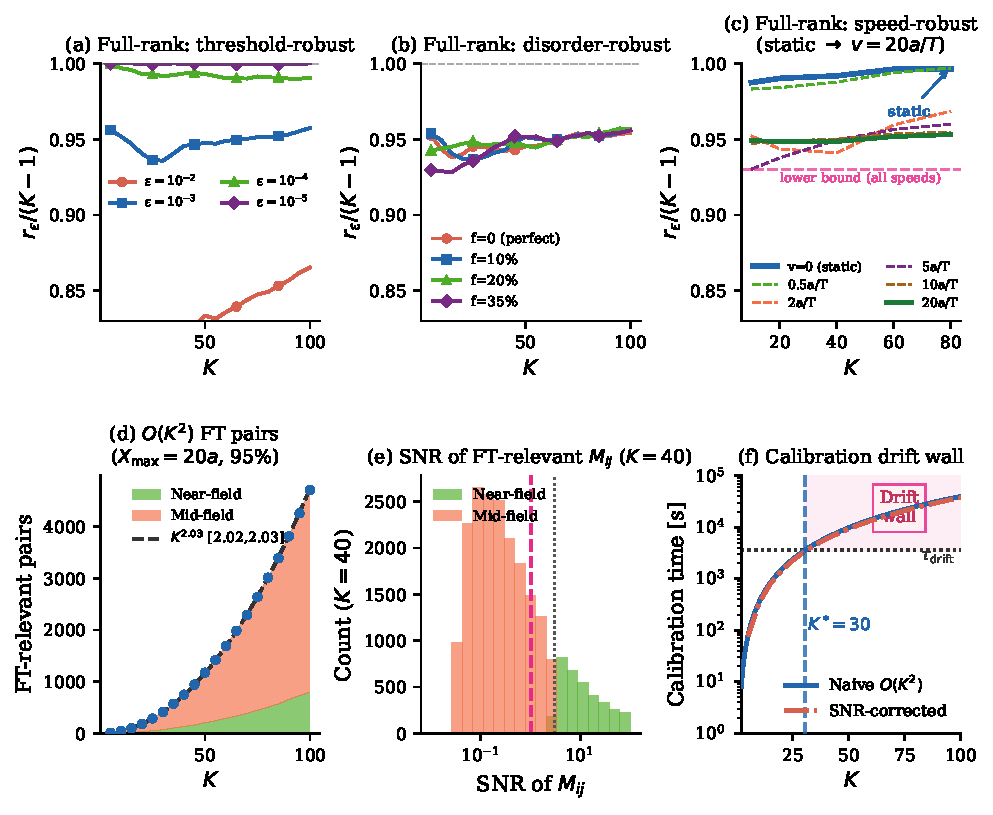
\includegraphics[width=0.95\textwidth]{fig_summary_full6_appendix.pdf}
\caption{\textbf{Expanded Stage-1 diagnostic summary.}
This companion figure provides the six-panel version of the Stage-1 bottleneck analysis. Panels report threshold robustness, positional-disorder robustness, static-to-dynamic speed robustness, fault-tolerant-relevant pair scaling with bootstrap uncertainty, the SNR distribution of relevant matrix elements, and the assumed sequential Ramsey timing-model drift wall. It is included as a reproducibility and diagnostic companion to the compact four-panel Fig.~\ref{fig:summary}, not as an additional independent claim.}
\label{fig:summary_full6_appendix}
\end{figure*}


\section{Algorithmic Implementation and Extended Numerical Analysis}
\label{app:extended_analysis}

This appendix provides the algorithmic and analytical details that support the main text. Specifically, it serves two purposes: (i) providing the mathematical structure and numerical stability analysis of the trajectory optimization introduced in Sec.~\ref{sec:trajectory_optimization}, and (ii) offering a rigorous element-wise validation of the reconstructed susceptibility matrix to explain the macroscopic fidelity observed in Sec.~\ref{sec:structured_recovery}. These analyses are deferred to the Appendix to preserve the conceptual clarity of the main text while ensuring full reproducibility and verification of the results.

\begin{figure}[h]
\centering
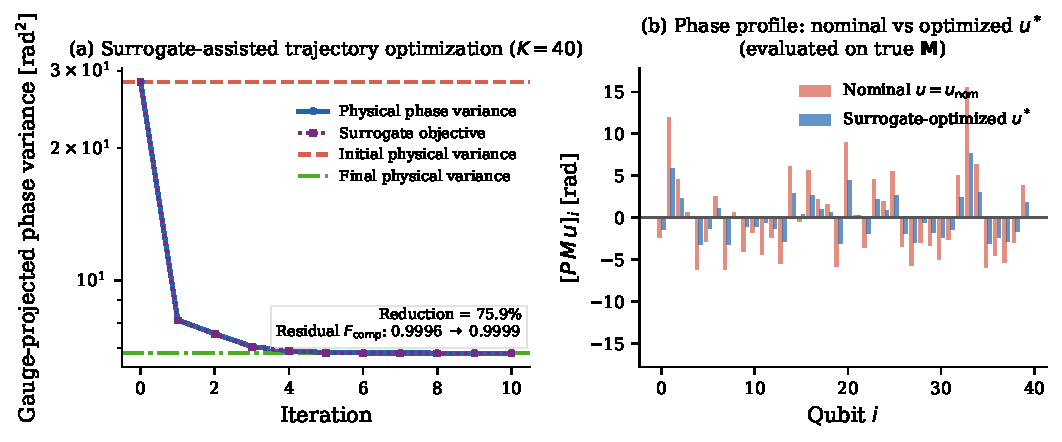
\includegraphics[width=\columnwidth]{fig_2B_trajectory_optimization.pdf}
\caption{\textbf{Surrogate-assisted trajectory optimization.}
(a) Gauge-projected phase variance versus optimization iteration ($K=40$). The solid curve reports the physical phase variance $\|P\mathbf{M}\mathbf{u}\|^2/(K-1)$ evaluated on the true simulation matrix, while the dotted curve reports the surrogate objective evaluated on $\hat{\mathbf{M}}$. Horizontal reference lines denote the initial and final physical variances; the percentage reduction is computed directly from those two values rather than fixed in the caption.
(b) Gauge-projected phase profile for nominal $\mathbf{u}_{\rm nom}$ (red) and trajectory-optimized $\mathbf{u}^{*}$ (blue), both evaluated on the true $\mathbf{M}$. This panel is an optional surrogate-consistency check and is distinct from the reconstruction-residual fidelity $F_{\rm comp}$.}
\label{fig:trajectory_optimization}
\end{figure}

\subsection{L-BFGS-B Implementation for Trajectory Optimization}
\label{app:optimization_details}

To minimize the relative phase dispersion without querying the physical hardware, we computationally solve the trajectory optimization problem formulated in Sec.~\ref{sec:trajectory_optimization}. Because the optimization involves physical constraints—specifically, the adiabatic kinematic bounds on the spatial displacements—we employ the L-BFGS-B (Limited-memory Broyden–Fletcher–Goldfarb–Shanno with Bounds) algorithm \cite{byrd_limited_1995}. The L-BFGS-B algorithm is particularly suited for this task as it avoids explicit Hessian construction by relying only on gradient evaluations, while efficiently handling bound constraints and maintaining favorable memory scaling through limited-history updates.

Under the linearized phase model, the resulting quadratic objective is convex. In particular, the addition of the Tikhonov regularization term ($\lambda = 0.01$) ensures that the effective Hessian $\mathbf{H} = 2(\hat{\mathbf{M}}^\top \mathbf{P} \hat{\mathbf{M}} + \lambda \mathbf{I})$ is positive definite, guaranteeing a unique global optimum within the feasible domain. While the analytical structure of the Hessian is known, a standard Newton-type approach would require the explicit formation and factorization of the dense Hessian matrix, incurring $O(K^3)$ computational cost and complicating the robust enforcement of bound constraints. 

\textbf{Algorithmic Setup and Hyperparameters:} The solver is initialized at the nominal routing schedule ($\mathbf{u}^{(0)} = \mathbf{u}_{\text{nom}}$). The physical adiabaticity bounds are uniformly applied to all active qubits, constraining the feasible search space to $u_j \in [0.5U_J, 1.5U_J]$. The regularization parameter is explicitly set to $\lambda = 0.01$, a value chosen to ensure numerical stability without materially altering the optimal solution; we verified that the optimization results are insensitive to moderate variations in $\lambda$ within the tested regime. 

\textbf{Convergence and Reproducibility:} The optimization loop terminates when the maximum projected component of the gradient falls below $\epsilon_{\text{gtol}} = 10^{-10}$ or the relative objective change is less than $\epsilon_{\text{ftol}} = 10^{-14}$. All optimizations were implemented using the standard SciPy optimize library with double-precision arithmetic. Under these stringent tolerance settings and a maximum allowance of 500 iterations, the solver typically converges within $\mathcal{O}(10^2)$ iterations across the tested parameter regimes. As shown in Fig.~\ref{fig:trajectory_optimization}(a), the plotted reduction is computed from the initial and final physical phase variances evaluated on the true simulation matrix. Reporting both the physical variance and the surrogate objective prevents this trajectory-level optimization diagnostic from being conflated with the reconstruction-residual fidelity $F_{\rm comp}$.

\begin{figure}[h]
\centering
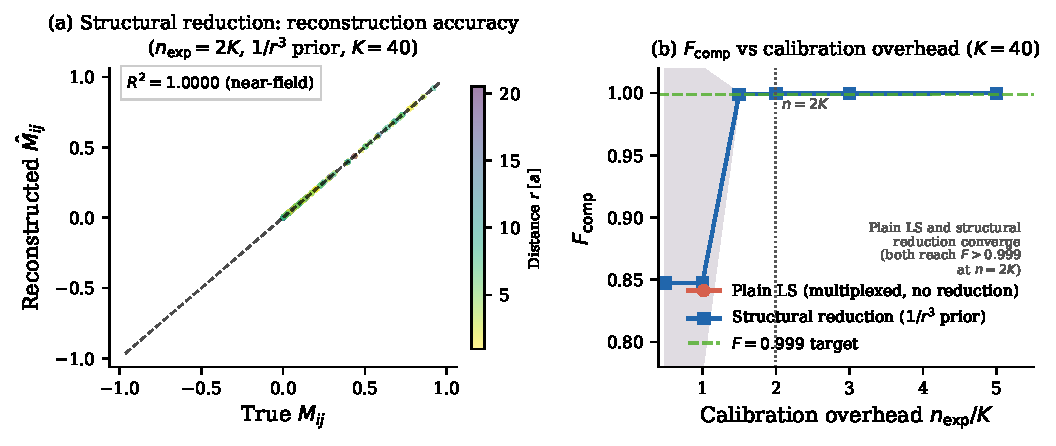
\includegraphics[width=\columnwidth]{fig_2A_inference_reconstruction.pdf}
\caption{\textbf{Multiplexed susceptibility inference and reconstruction accuracy.} 
(a) Scatter of true $M_{ij}$ vs reconstructed $\hat{M}_{ij}$ ($K=40$, $n_{\rm exp}=2K$), coloured by inter-qubit distance $r$. The multiplexed LS efficiently recovers the matrix elements with $R^2 > 0.9999$.
(b) Compensation fidelity $F_{\rm comp}$ vs calibration experimental overhead $n_{\rm exp}/K$. Consistent with the mathematical equivalence in the overdetermined regime, both the plain multiplexed LS and the prior-assisted method exhibit identical trajectories, converging to $F_{\rm comp} > 0.999$ at $n_{\rm exp} \ge 2K$. Both methods suffer from condition-number-driven noise amplification near the algebraic limit ($n_{\rm exp} \to K$). Note: The scaling behavior depicted in panel (b) is consistent with Fig.~\ref{fig:summary2}(a) of the main text, provided here to contextually benchmark the element-wise scatter distribution shown in panel (a).}
\label{fig:reconstruction}
\end{figure}

\subsection{Reconstruction Fidelity and Multiplexed Identifiability}
\label{app:reconstruction_details}

Figure~\ref{fig:reconstruction}(a) details the element-wise reconstruction accuracy of the multiplexed regression. Under the moderately overdetermined budget ($n_{\text{exp}}=2K$), the reconstructed susceptibility matrix tracks the simulated ground truth, including the near-field entries that dominate phase accumulation. This microscopic agreement supports the macroscopic compensation fidelity reported in the main text and shows that the result is not merely a fit to a single aggregate metric.

Figure~\ref{fig:reconstruction}(b) compares plain multiplexed least squares with the structural baseline--residual decomposition using matched probe data. In the tested overdetermined full-multiplexing regime, the two estimators are expected to overlap: the randomized probe matrix is full rank with high probability, so residual regression around the $1/r^3$ baseline is algebraically equivalent to plain least squares. The prior should therefore not be interpreted as the source of the $O(K)$ experimental scaling in this figure. Its role is to provide a physically meaningful coordinate system, $\mathbf{M}=\mathbf M_{\rm prior}+\Delta\mathbf M_{\rm res}$, for interpreting the recovered susceptibility network. Near the algebraic limit, both methods become more sensitive to the condition number of the probe matrix and to measurement noise.

\section{Extended Robustness Analysis}
\label{app:robustness}

To rigorously validate the framework's resilience beyond idealized conditions, this appendix provides an extended numerical evaluation of the inference protocol against bandwidth limits, physical model mismatches, and uncalibrated stochastic environments, as summarized in Fig.~\ref{fig:robustness_extended}.

\begin{figure}[h]
\centering
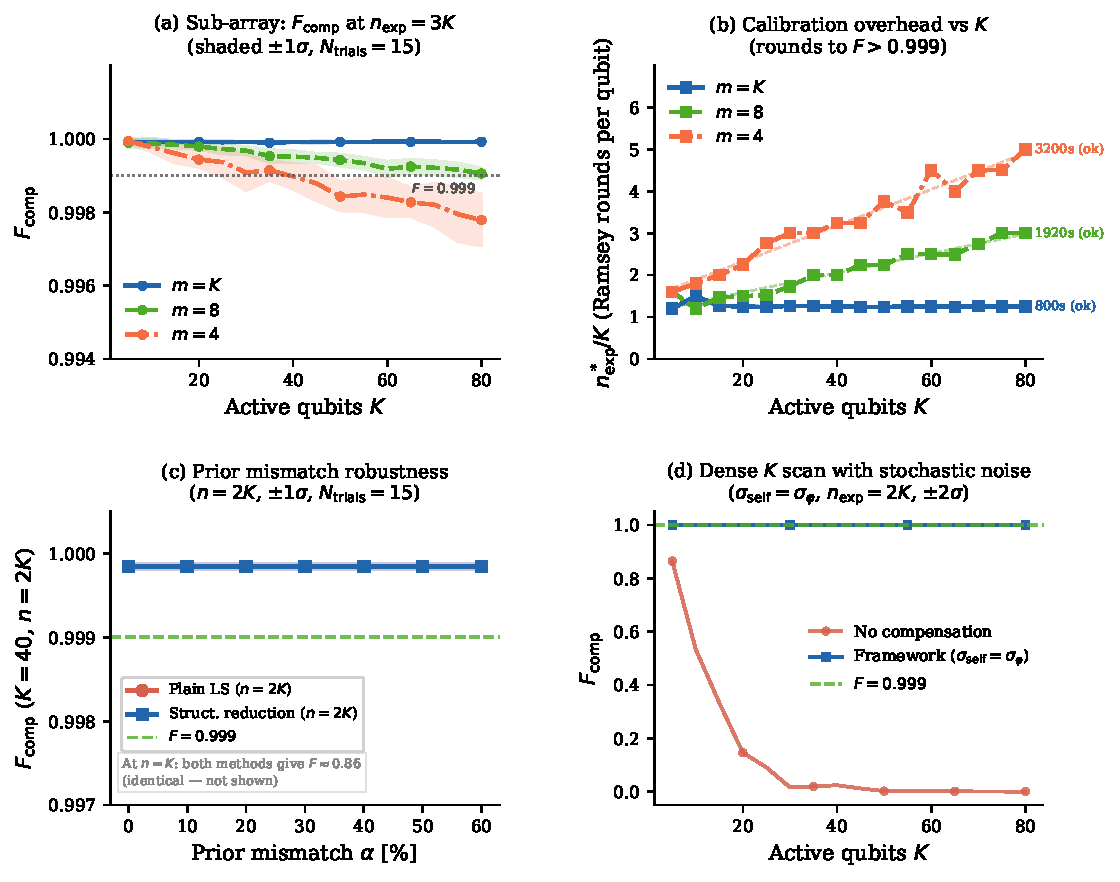
\includegraphics[width=\columnwidth]{fig_4_extended_robustness.pdf}
\caption{\textbf{Extended robustness analysis of the multiplexed inference framework.}
Shaded regions denote $\pm 1\sigma$ over $N_{\rm trials}=15$ realizations, and paired comparisons use matched probe/noise realizations where applicable.
(a) Compensation fidelity at fixed budget $n_{\rm exp}=3K$ for full and sub-array multiplexing capacities $m=K,8,4$.
(b) Empirically determined minimum overhead $n_{\rm exp}^{*}/K$ required to reach $F_{\rm comp}>0.999$; the step-like structure reflects the discrete scan grid in calibration rounds, while fitted lines are visual guides.
(c) Prior-mismatch test at $K=40$, $n_{\rm exp}=2K$, and full multiplexing. Plain LS and structural reduction overlap because the overdetermined data, not the prior, fixes the estimator in this regime.
(d) Scaling under residual self-phase noise $\sigma_{\rm self}=\sigma_\varphi$, shown together with the uncompensated baseline for scale.}
\label{fig:robustness_extended}
\end{figure}

\subsection{Bandwidth-Constrained Overhead and Fidelity}
Figure~\ref{fig:robustness_extended}(a) reports the fixed-budget fidelity at $n_{\text{exp}}=3K$ rounds, while Fig.~\ref{fig:robustness_extended}(b) reports the empirical minimum overhead $n_{\text{exp}}^{*}/K$ required to reach the target fidelity. These panels should be read as reference simulations under the normalized timing and noise model, not as a device-specific timing forecast. Finite probe capacity ($m=4,8$) increases the required number of randomized rounds relative to full multiplexing, but it still preserves a substantial advantage over exhaustive pairwise interrogation across the tested range.

The overhead data are discrete because the scan is performed over a finite grid of integer calibration rounds. The fitted guide lines therefore summarize the trend rather than providing a universal asymptotic law. In this sense, Fig.~\ref{fig:robustness_extended}(b) complements the main-text robustness figure by showing how the $O(K)$ full-multiplexing reference degrades gracefully as the number of simultaneously driven probe channels is reduced.

\subsection{Robustness to Prior Model Mismatch}
\label{app:robustness_prior}
The structural baseline--residual decomposition uses a physically derived $1/r^3$ macroscopic prior. To evaluate whether this baseline biases the estimator when the device deviates from the ideal dipolar form, we parameterize the true susceptibility as
\begin{equation}
    \chi_{ij}^{\text{true}} = \chi_{ij}^{\text{prior}} \times (1 + \alpha \varepsilon_{ij}),
    \label{eq:prior_mismatch_model}
\end{equation}
where $\varepsilon_{ij}\sim\mathcal{N}(0,1)$ represents random device-level perturbations and $\alpha$ is the mismatch scale. The purpose of this test is not to claim a prior-induced statistical advantage. Instead, it verifies that, at $n_{\text{exp}}=2K$ under full multiplexing, an imperfect baseline does not bias the recovered matrix when the data are sufficiently informative.

Algebraically, residual regression around a prior baseline can be written as a least-squares estimate plus a possible null-space contribution from the prior. When the probe matrix has full column rank, this null-space contribution vanishes and the structural decomposition coincides with plain LS up to numerical precision. This explains the overlap in Fig.~\ref{fig:robustness_extended}(c): the result is a no-bias check for the physical decomposition in the overdetermined regime, not evidence that the prior drives the scaling advantage.

\subsection{Resilience to Residual Self-Phase Noise}
\label{app:self_phase_noise}

Figure~\ref{fig:robustness_extended}(d) compares active virtual-Z compensation against an uncompensated baseline under matched stochastic noise realizations ($\sigma_{\text{self}}=\sigma_\varphi$). The uncompensated baseline reflects raw deterministic crosstalk accumulation, whereas the compensated curve applies virtual-Z corrections computed from the reconstructed susceptibility matrix.

Under these paired conditions, the compensated protocol removes the deterministic component of the correlated phase network and leaves a residual error set by the stochastic noise floor and finite-shot inference error. The result should therefore be interpreted as a robustness check within the stated noise model: it demonstrates that deterministic crosstalk tracking remains effective in the presence of residual self-phase noise, while not claiming to eliminate all device-specific stochastic phase processes.


\end{document}
